\documentclass[10pt]{book}
\raggedbottom

\usepackage{amsmath}
\usepackage{amssymb}
\usepackage{amsfonts}
\usepackage[mathscr]{euscript}


%	%	%	%	%	%
%	Look & Layout	%
%	%	%	%	%	%

\usepackage[margin=1in]{geometry}

\usepackage{titlesec}
\titleformat{\chapter}[hang]{\Large\bfseries}{\thechapter\hspace{1em}}{0pt}{\Large\bfseries} % Compact Chapter title
\titlespacing{\chapter}{0pt}{0pt}{0pt}	% Eliminate space before/after chapter
\usepackage{fancyhdr}
\pagestyle{fancy}
\everymath{\displaystyle}
\usepackage{multicol}
\setlength\columnsep{3em}
\raggedcolumns
\usepackage[inline,shortlabels]{enumitem} % For inline lists

\usepackage{mdframed}
\newenvironment{boxthm}{\begin{mdframed}[backgroundcolor=gray!30,nobreak=true]}{\end{mdframed}}
\newenvironment{boxdef}{\begin{mdframed}[backgroundcolor=gray!30,linewidth=0pt,nobreak=true]}{\end{mdframed}}


%	%	%	%	%	%	%	%	%	%	%
%	Systems of Equations and Matrices	%
%	%	%	%	%	%	%	%	%	%	%

\usepackage{systeme}
%\syslineskipcoeff{1.2}\setlength{\tabskip}{3pt}
%\systeme{
%	2x  +   y  +  3z  =  10,
%	x  +   y  +   z  =   6,
%	x  +  3y  +  2z  =  13}

% Right align RHS
\makeatletter
\def\SYS@makesyspreamble@i#1{%
	\ifnum#1<\SYS@preamblenum
	\SYS@addtotok\SYS@systempreamble{\hfil$##$&\hfil$##$&}% 
	\expandafter\SYS@makesyspreamble@i\expandafter{\number\numexpr#1+\@ne\expandafter}%
	\else
	\SYS@addtotok\SYS@systempreamble{\hfil$##$&$##$&\hfil$##$\null}% 
	\ifSYS@extracol
	\SYS@addtotok\SYS@systempreamble{&\SYS@extracolstart##\SYS@extracolend\hfil\null}% 
	\fi
	\SYS@addtotok\SYS@systempreamble{\cr\SYS@strutup}% 
	\fi
}
\makeatother

% Remove brace from systeme
\syscodeextracol{\quad\hfill}{\hfill}
\sysdelim..


% Add alignment to matrices - default to right [r]
\makeatletter
\renewcommand*\env@matrix[1][r]{\hskip -\arraycolsep
	\let\@ifnextchar\new@ifnextchar
	\array{*\c@MaxMatrixCols #1}}
\makeatother


%	%	%	%	%
%	pgf Plots	%
%	%	%	%	%

\usepackage{tikz}
\usetikzlibrary{matrix,positioning}
\usepackage{pgfplots}
\pgfplotsset{compat=1.11}	% As of 1.11, you may write tikz coordinates as (2,1)
							% rather than having to type (axis cs:2,1)


%	%	%	%	% 	%
%	My Commands		%
%	%	%	%	%	%

\newcommand{\N}{\mathbb{N}}
\newcommand{\R}{\mathbb{R}}
\newcommand{\Poly}{\mathbb{P}}
\newcommand{\B}{\mathscr{B}}
\newcommand{\C}{\mathscr{C}}
\newcommand{\E}{\mathscr{E}}
\newcommand{\vect}[1]{\ensuremath{\boldsymbol{\mathbf{#1}}}}
\DeclareMathOperator{\Span}{Span}
\DeclareMathOperator{\adj}{adj}
\DeclareMathOperator{\Nul}{Nul}
\DeclareMathOperator{\Col}{Col}
\DeclareMathOperator{\Row}{Row}
\DeclareMathOperator{\rank}{rank}
\DeclareMathOperator{\proj}{proj}
\DeclareMathOperator{\dist}{dist}
\DeclareMathOperator{\col}{col}
\DeclareMathOperator{\row}{row}

\newcommand{\Axb}{A\vect{x}=\vect{b}}
\newcommand{\Axz}{A\vect{x}=\vect{0}}
\newcommand{\Ax}{A\vect{x}}
\newcommand{\Tx}{T(\vect{x})}
\newcommand{\ve}[1]{\vect{e}_{#1}}
\newcommand{\Te}[1]{T(\ve{#1})}
\newcommand{\Tmap}[2]{T:\R^{#1}\to\R^{#2}}
\newcommand{\vectset}[3][v]{\{\vect{#1}_{#2},\ldots,\vect{#1}_{#3}\}}
\newcommand{\vectsetvp}{\{\vect{v}_1,\ldots,\vect{v}_p\}}
\newcommand{\vectB}[1][x]{[\vect{#1}]_\B}
\newcommand{\vectC}[1][x]{[\vect{#1}]_\C}
\newcommand{\CoC}[2]{\underset{#2\leftarrow #1}{P}}

\newcommand{\Axlx}{A\vect{x}=\lambda\vect{x}}

\newcommand{\yhat}{\hat{\vect{y}}}
\newcommand{\xhat}{\hat{\vect{x}}}
\newcommand{\bhat}{\hat{\vect{b}}}
\newcommand{\Axbhat}{A\xhat=\bhat}
\newcommand{\NormEq}{A^TA\vect{x} = A^T\vect{b}}


% Special Matrices
\newcommand{\RotMat}[1][\theta]{\begin{bmatrix}\cos#1&-\sin#1\\ \sin#1&\cos#1\end{bmatrix}}
\newcommand{\ReflectMatHorz}{\begin{bmatrix}1&0\\0&-1\end{bmatrix}}
\newcommand{\ReflectMatVert}{\begin{bmatrix}-1&0\\0&1\end{bmatrix}}
\newcommand{\ReflectMatDiag}{\begin{bmatrix}0&1\\1&0\end{bmatrix}}
\newcommand{\ReflectMatRevDiag}{\begin{bmatrix}0&-1\\-1&0\end{bmatrix}}
\newcommand{\ReflectMatOrigin}{\begin{bmatrix}-1&0\\0&-1\end{bmatrix}}
\newcommand{\ShearMatHorz}[1][k]{\begin{bmatrix}1&#1\\0&1\end{bmatrix}}
\newcommand{\ShearMatVert}[1][k]{\begin{bmatrix}1&0\\#1&1\end{bmatrix}}
\newcommand{\ExpandMatHorz}[1][k]{\begin{bmatrix}#1&0\\0&1\end{bmatrix}}
\newcommand{\ExpandMatVert}[1][k]{\begin{bmatrix}1&0\\0&#1\end{bmatrix}}
\newcommand{\ExpandMatBoth}[1][k]{\begin{bmatrix}#1&0\\0&#1\end{bmatrix}}
\newcommand{\ProjMatHorz}{\begin{bmatrix}1&0\\0&0\end{bmatrix}}
\newcommand{\ProjMatVert}{\begin{bmatrix}0&0\\0&1\end{bmatrix}}

\newcommand{\Iarb}{\begin{bmatrix}1&0&0&\cdots&0\\0&1&0&\cdots&0\\0&0&1&\cdots&0\\\vdots&\vdots&\vdots&\ddots&\vdots\\0&0&0&\cdots&1\end{bmatrix}}
\newcommand{\I}[1]{
	\ifnum#1=2 {\begin{bmatrix}1&0\\0&1\end{bmatrix}}
	\else\ifnum#1=3 {\begin{bmatrix}1&0&0\\0&1&0\\0&0&1\end{bmatrix}}
	\else\ifnum#1=4 {\begin{bmatrix}1&0&0&0\\0&1&0&0\\0&0&1&0\\0&0&0&1\end{bmatrix}}
	\else {I_n}
	\fi\fi\fi
	}

\begin{document}
\pagenumbering{gobble}

% SEC 1.1
\chapter{Linear Equations}
\chaptermark{Linear Equations}
\section{Systems of Linear Equations}
\begin{itemize}
	\item Linear Equations
		\begin{itemize}
			\item $a_1x_1 + a_2x_2 + \cdots + a_nx_n = b$
			\item Solution to a linear equation, $(s_1,s_2,\ldots,s_n)$
			\item Systems of linear equations, solution sets, and equivalent systems
		\end{itemize}
	\item Matrices
		\begin{itemize}
			\item Coefficient matrix and augmented matrix
			\item Size of a matrix, e.g. if $A$ is $3\times 5$, it has 3 rows and 5 columns
		\end{itemize}
	\item Elementary Row Operations (If the augmented matrices of two linear systems are row equivalent, then the two systems have the same solution set.)
		\begin{enumerate}
			\item Interchange: Interchange two rows
			\item Scale: Multiply all entries in a row by a nonzero scalar
			\item Replace: Replace a row with the sum of itself and a multiple of another row
		\end{enumerate}
	\item Consistent vs Inconsistent Systems
		\begin{itemize}
			\item Consistent: the system has one or infinitely many solutions
			\item Inconsistent: the system has no solutions
		\end{itemize}
	\item Fundamental Questions About Linear Systems
		\begin{itemize}
			\item Existence: Does the system have at least one solution?
			\item Uniqueness: When there is a solution, is it unique? (Or are there infinitely many solutions?)
		\end{itemize}
\end{itemize}

% SEC 1.2
\section{Row Reduction and Echelon Forms}
\begin{itemize}
	\item Row Echelon Form and Reduced Row Echelon Form of a Matrix (Theorem 1)
		\begin{itemize}
			\item REF is enough to tell you if the system is consistent/inconsistent
			\item REF is enough to determine pivot positions---this tells you which variables are basic/free
			\item RREF is unique for equivalent systems and will give you a general solution
		\end{itemize}
	\item Leading Entries, Pivot Positions, and Pivot Columns (Theorem 2)
	\item Basic Variables vs Free Variables (Theorem 2)
\end{itemize}
\begin{boxthm}
	\textbf{Theorem 1.1.}
	\textbf{Uniqueness of the Reduced Echelon Form} \\
	Each matrix is row equivalent to one, and only one, reduced echelon matrix.
\end{boxthm}
\begin{boxthm}
	\textbf{Theorem 1.2.}
	\textbf{Existence and Uniqueness Theorem} \\
	A linear system is consistent if, and only if, the rightmost column of the augmented matrix is \textit{not} a pivot column---that is, if, and only if, an echelon form of the augmented matrix has \textit{no} row of the form
	$$ \begin{bmatrix}0 & \cdots & 0 & b\end{bmatrix} \qquad \text{with $b$ nonzero}.$$
	If a linear system is consistent, then the solution set contains either 
	\begin{enumerate*}[(i)]
		\item a unique solution, when there are no free variables, or
		\item infinitely many solutions, when there is at least one free variable.
	\end{enumerate*}
\end{boxthm}

\pagebreak

\begin{boxdef}
	\textbf{Using Row Reduction to Solve a Linear System}
	\begin{enumerate}
		\item Write the augmented matrix of the system.
		\item Use the row reduction algorithm to obtain an equivalent augmented matrix in echelon form. Decide whether the system is consistent. If there is no solution, stop; otherwise, go to the next step
		\item Continue row reduction to obtain the reduced echelon form.
		\item Write the system of equations corresponding to the matrix obtained in the previous step
		\item Rewrite each nonzero equation from the previous step so that its one basic variable is expressed in terms of the any free variables appearing in the equation.
	\end{enumerate}
\end{boxdef}

% SEC 1.3
\section{Vector Equations}
\begin{itemize}
	\item $\R^2,\R^3,\ldots,\R^n$
	\item Vectors
		\begin{itemize}
			\item Vector Operations
				\begin{itemize}
					\item Addition: $\vect{v}+\vect{u}$
					\item Scalar Multiples: $c\vect{u}$
					\item Other algebraic properties (pg. 27)
				\end{itemize}
			\item Geometric interpretation (vectors as points in $\R^n$)
			\item Parallelogram Rule for Addition
				\begin{boxdef}
					If $\vect{u}$ and $\vect{v}$ in $\R^2$ are represented as points in the plane, then $\vect{u}+\vect{v}$ corresponds to the fourth vertex of the parallelogram whose other vertices are $\vect{u}$, $\vect{0}$, and $\vect{v}$.
				\end{boxdef}
		\end{itemize}
	\item Linear Combinations
		\begin{itemize}
			\item $c_1\vect{v_1}+c_2\vect{v_2}+\cdots+c_n\vect{v_n}=\vect{b}$
			\item Weights
		\end{itemize}
	\item Vector Equations and Augmented Matrices
		\begin{boxdef}
			A vector equation $x_1\vect{a_1}+x_2\vect{a_2}+\cdots+x_3\vect{a_n}=\vect{b}$ has the same solution set as the linear system whose augmented matrix is $\begin{bmatrix}\vect{a_1}&\vect{a_2}&\cdots&\vect{a_n}&\vect{b}\end{bmatrix}$.
		\end{boxdef}
	\item Span
		\begin{boxdef}
			If $\vect{v_1},\vect{v_2},\ldots,\vect{v_n}$ are in $\R^n$, $\Span\{\vect{v_1},\vect{v_2},\ldots,\vect{v_n}\}$ is the set of all linear combinations of $\vect{v_1},\vect{v_2},\ldots,\vect{v_n}$. It is called the \textbf{subset of $\boldsymbol{\R^n}$ spanned by $\vect{v_1},\vect{v_2},\ldots,\vect{v_n}$}. In other words, $\Span\{\vect{v_1},\vect{v_2},\ldots,\vect{v_n}\}$ is the set of all vectors that can be written in the form $c_1\vect{v_1}+c_2\vect{v_2}+\cdots+c_n\vect{v_n}$ with $c_1,\ldots,c_n$ scalars.
		\end{boxdef}
		\begin{itemize}
			\item Geometric description of $\Span\{\vect{u}\}$ and $\Span\{\vect{u},\vect{v}\}$
		\end{itemize}
	\item Equivalent Questions
		\begin{align*}
		\vect{b}\in\Span\{\vect{v_1},\vect{v_2},\ldots,\vect{v_n}\}
			&& \text{Is $\vect{b}$ in the span of $\vect{v_1},\vect{v_2},\ldots,\vect{v_n}$?} \\
		x_1\vect{a_1}+x_2\vect{a_2}+\cdots+x_3\vect{a_n}=\vect{b}
			&& \text{Does this vector equation have a solution?} \\
		\begin{bmatrix}\vect{v_1}&\cdots&\vect{v_n}&\vect{b}\end{bmatrix}
			&& \text{Is the corresponding linear system consistent?}
		\end{align*}
\end{itemize}


\newpage


% SEC 1.4
\section{The Matrix Equation $\boldsymbol{Ax=b}$}
\begin{itemize}
	\item Matrix-Vector Product: $A\vect{x}$
		\begin{itemize}
			\item Linear combination of the columns of $A$
			\begin{boxdef}
				If $A$ is an $m\times n$ matrix with columns $\vect{a}_1,\ldots,\vect{a}_n$, and if $\vect{x}$ is in $\R^n$, then the product of $A$ and $\vect{x}$, denoted by $A\vect{x}$ is the linear combination of the columns of $A$ using the corresponding entries in $\vect{x}$ as weights:
				$$ A\vect{x} =
				\begin{bmatrix}\vect{a}_1&\vect{a}_2&\cdots&\vect{a}_n\end{bmatrix}
				\begin{bmatrix}[c]x_1\\\vdots\\x_n\end{bmatrix} =
				x_1\vect{a}_1 + x_2\vect{a}_2 + \cdots + x_n\vect{a}_n $$
			\end{boxdef}
			\item Row-vector rule
			\begin{boxdef}
				If the product $A\vect{x}$ is defined, then the $i$th entry in $A\vect{x}$ is the sum of the products of corresponding entries from row $i$ of $A$ and from the vector $\vect{x}$.
			\end{boxdef}
			\item Properties of matrix-vector products (Theorem 5)
		\end{itemize}
	\item Matrix Equation: $A\vect{x}=\vect{b}$
		\begin{itemize}
			\item 3 equivalent ways to view the problem (Theorem 3)
			\begin{align*}
			\text{Sys. of Linear Eq.}&&&&
			\text{Vector Equation}&&&&
			\text{Matrix Equation} \\
			\systeme{x_1+2x_2-x_3=4,-5x_2+3x_3=1}&
			&\Longleftrightarrow&&
			x_1\begin{bmatrix}1\\0\end{bmatrix} + x_2\begin{bmatrix}2\\-5\end{bmatrix} + x_3\begin{bmatrix}-1\\3\end{bmatrix} &=
			\begin{bmatrix}4\\1\end{bmatrix}
			&\Longleftrightarrow&&
			\begin{bmatrix}1&2&-1\\0&-5&3\end{bmatrix}
			\begin{bmatrix}x_1\\x_2\\x_3\end{bmatrix} &=
			\begin{bmatrix}4\\1\end{bmatrix}
			\end{align*}
			\item Existence of solutions for $A\vect{x}=\vect{b}$ (Theorem 4)
				\begin{itemize}
					\item $A\vect{x}=\vect{b}$ has a solution if, and only if, $\vect{b}$ is a linear combination of the columns of $A$
					\item If the columns of $A$ span all of $\R^m$, then $A\vect{x}=\vect{b}$ has a solution for any choice of $\vect{b}\in\R^m$
				\end{itemize}
		\end{itemize}
	\item The Identity Matrix, $I$ or $I_n$.
\end{itemize}
\begin{boxthm}
	\textbf{Theorem 1.3.} \\
	If $A$ is an $m\times n$ matrix with columns $\vect{a}_1,\ldots,\vect{a}_n$, and if $\vect{b}$ is in $\R^m$, the matrix equation $A\vect{x}=\vect{b}$ has the same solutions set as the vector equation $x_1\vect{a}_1+x_2\vect{a}_2+\cdots+x_n\vect{a}_n=\vect{b}$ which, in turn, has the same solution set as the system of linear equations whose augmented matrix is $\begin{bmatrix}\vect{a}_1&\vect{a}_2&\cdots&\vect{a}_n&\vect{b}\end{bmatrix}$.
\end{boxthm}
\begin{boxthm}
	\textbf{Theorem 1.4.} \\
	Let $A$ be an $m\times n$ matrix. Then the following statements are logically equivalent.
	\begin{enumerate}[(a)]\itemsep0em 
		\item For each $\vect{b}$ in $\R^m$, the equation $A\vect{x}=\vect{b}$ has a solution.
		\item Each $\vect{b}$ in $\R^m$ is a linear combination of the columns of $A$.
		\item The columns of $A$ span $\R^m$.
		\item $A$ has a pivot position in every row.
	\end{enumerate}
\end{boxthm}
\begin{boxthm}
	\textbf{Theorem 1.5.} \\
	If $A$ is an $m\times n$ matrix, $\vect{u}$ and $\vect{v}$ are vectors in $\R^n$, and $c$ is a scalar, then:
	\begin{enumerate}[(a)]\itemsep0em 
		\item $A(\vect{u}+\vect{v}) = A\vect{u} + A\vect{v}$, and
		\item $A(c\vect{u}) = c(A\vect{u})$.
	\end{enumerate}
\end{boxthm}


% SEC 1.5
\section{Solution Sets of Linear Systems}
\begin{itemize}
	\item Homogeneous Linear System: $A\vect{x}=\vect{0}$
		\begin{itemize}
			\item Always has the trivial solution, $\vect{x}=\vect{0}$
			\item Existence of nontrivial solutions?
			\begin{boxdef}
				The homogeneous equation $A\vect{x}=\vect{0}$ has a nontrivial solution if, and only if, the equation has at least one free variable.
			\end{boxdef}
		\end{itemize}
	\item Implicit vs Explicit Descriptions of Solution Sets
		\begin{itemize}
			\item Implicit: e.g. Equation of a plane
			\item Explicit: Parametric vector form of the solution set
				\begin{boxdef}
					To find the solution fo a system of equations in \textbf{parametric vector form}, follow these steps:
					\begin{enumerate}
						\item Row reduce augmented matrix to RREF.
						\item Express basic variables in terms of free variables.
						\item Write the solution $\vect{x}$ as a vector whose entries depend on the free variables.
						\item Decompose $\vect{x}$ into a linear combination of vectors using free variables as parameters.
					\end{enumerate}
				\end{boxdef}
		\end{itemize}
	\item Nonhomogeneous Linear System: $A\vect{x}=\vect{b}$, where $\vect{b}\neq\vect{0}$
		\begin{itemize}
			\item Geometric relationship between solution set of $A\vect{x}=\vect{b}$ and solution set of $A\vect{x}=\vect{0}$ (Theorem 6)
		\end{itemize}
\end{itemize}

\begin{boxthm}
	\textbf{Theorem 1.6.} \\
	Suppose the equation $A\vect{x}=\vect{b}$ is consistent for some given $\vect{b}$, and let $\vect{p}$ be a solution. Then the solution set of $A\vect{x}=\vect{b}$ is the set of all vectors of the form $\vect{w}=\vect{p}+\vect{v}_h$, where $\vect{v}_h$ can be any solution of the homogeneous equation $A\vect{x}=\vect{0}$.
\end{boxthm}
\vfill


% SEC 1.6
\section{Applications of Linear Systems} (not on Test 1)
\begin{itemize}
	\item A Homogeneous System in Economics
		\begin{itemize}
			\item Find equilibrium prices in primitive economic models using homogeneous systems
		\end{itemize}
	\item Balancing Chemical Equations
	\begin{itemize}
		\item Balance chemical equations using integer solutions to systems of linear equations
	\end{itemize}
	\item Network Flow
	\begin{itemize}
		\item Traffic flow on a network of roads
	\end{itemize}
\end{itemize}
\vfill


\newpage


% SEC 1.7
\section{Linear Independence}
\begin{itemize}
\item Linearly Independent
\begin{boxdef}
	An indexed set of vectors $\{\vect{v}_1,\ldots,\vect{v}_p\}$ in $\R^n$ is said to be \textbf{linearly independent} if the vector equation
	$$ x_1\vect{v}_1 + x_2\vect{v}_2 + \cdots + x_p\vect{v}_p = \vect{0} $$
	has only the trivial solution. The set $\{\vect{v}_1,\ldots,\vect{v}_p\}$ is said to be \textbf{linearly dependent} if there exist weights $c_1,\ldots,c_p$ not all zero, such that
	$$ c_1\vect{v}_1 + c_2\vect{v}_2 + \cdots + c_p\vect{v}_p = \vect{0}. $$
\end{boxdef}
\item Linear Independence of Matrix Columns
\begin{boxdef}
	The columns of a matrix $A$ are linearly independent if, and only if, the equation $\Axz$ has \emph{only} the trivial solution.
\end{boxdef}
\item Sets of One or Two Vectors
	\begin{itemize}
		\item A set with just one nonzero vector is linearly independent, e.g. $\{\vect{u}\}$ with $\vect{u}\neq\vect{0}$
		\item The zero vector is linearly dependent, $\{\vect{0}\}$
		\item A set of two vectors is linearly dependent if one is a scalar multiple of the other, e.g. $\{\vect{u},-3\vect{u}\}$
	\end{itemize}
\item Sets of Two or More Vectors (Theorems 7, 8, and 9)
\end{itemize}

\begin{boxthm}
	\textbf{Theorem 1.7.}
	\textbf{Characterization of Linearly Independent Sets} \\
	An indexed set $S=\{\vect{v}_1,\ldots,\vect{v}_p\}$ of two or more vectors is linearly dependent if, and only if, at least one of the vectors in $S$ is a linear combination of the others. In fact, if $S$ is linearly dependent and $\vect{v}_1\neq\vect{0}$ then some $\vect{v}_j$ (with $j>1$) is a linear combination of the preceding vectors, $\vect{v}_1,\ldots,\vect{v}_{j-1}$.
\end{boxthm}
\begin{boxthm}
	\textbf{Theorem 1.8.} \\
	If a set contains more vectors than there are entries in each vector, then the set is linearly dependent. That is, any set $\{\vect{v}_1,\ldots,\vect{v}_p\}$ in $\R^n$ is linearly dependent if $p>n$.
\end{boxthm}
\begin{boxthm}
	\textbf{Theorem 1.9.} \\
	If a set $S=\{\vect{v}_1,\ldots,\vect{v}_p\}$ in $\R^n$ contains the zero vector, then the set is linearly dependent.
\end{boxthm}


\newpage


% SEC 1.8
\section{Introduction to Linear Transformations}
\begin{itemize}
	\item Transformations
%		\begin{itemize}
%			\item Transformation, function, or mapping
%			\item Domain and Codomain
%			\item Image and Range
%		\end{itemize}
		\begin{boxdef}
			A \textbf{transformation} (or \textbf{function} or \textbf{mapping}) $T$ from $\R^n$ to $\R^m$ is a rule that assigns to each vector in $\R^n$ a vector $T(\vect{x})$ in $\R^m$. The set $\R^n$ is called the \textbf{domain} of $T$, and $\R^m$ is called the \textbf{codomain} of $T$. We use the notation $T:\R^n\to\R^m$. For $\vect{x}\in\R^n$, the vector $T(\vect{x})$ is called the \textbf{image} of $\vect{x}$ (under the action of $T$). The set of all images $T(\vect{x})$ is called the \textbf{range} of $T$.
		\end{boxdef}
	\item Matrix Transformations
		\begin{itemize}
			\item Define $T:\R^n\to\R^m$ by $T(\vect{x})=\Ax$
			\item Connection between rows and cols of $A$ and domain, codomain, and range of $T$ when $T(\vect{x})=\Ax$
			\item Some examples of matrix transformations
				\begin{itemize}
					\item Projection
					\item Shear
					\item Rotation
					\item Reflection
					\item Contraction
					\item Dilation
				\end{itemize}
				Note: Although the last two examples, contraction and dilation, were not expressed as matrix transformations in this section, they can easily be written as such (see example 2 in section 1.9).
		\end{itemize}
	\item Linear Transformations
		\begin{boxdef}
			A transformation $T$ is \textbf{linear} if:
			\begin{enumerate}[(i)]
				\item $T(\vect{u}+\vect{v}) = T(\vect{u})+T(\vect{v})$ for all $\vect{u}$ and $\vect{v}$ in the domain of $T$.
				\item $T(c\vect{u}) = cT(\vect{u})$ for all scalars $c$ and all $\vect{u}$ in the domain of $T$.
			\end{enumerate}
		\end{boxdef}
		\begin{boxdef}
			If $T$ is a linear transformation, then
			\begin{enumerate}[(i)]
				\item $T(\vect{0})=\vect{0}$
				\item $T(c\vect{u}+d\vect{v}) = cT(\vect{u})+dT(\vect{v})$ for all scalars $c,d$ and all vectors  $\vect{u},\vect{v}$ in the domain of $T$.
			\end{enumerate}
			Note: to check if a transformation $T$ is linear, you only need to show that (ii) is true.
		\end{boxdef}
\end{itemize}


\newpage


% SEC 1.9
\section{The Matrix of a Linear Transformation}
\begin{itemize}
	\item Matrix Transformations
		\begin{itemize}
			\item Any linear transformation from $\R^n\to\R^m$ is a matrix transformation, $\vect{x}\mapsto A\vect{x}$
			\item The \textbf{standard matrix} for a linear transformation $T:\R^n\to\R^m$ (Theorem 10)
		\end{itemize}
	\item Geometric Linear Transformations of $\R^2$ (see charts in section 1.9)
		\begin{multicols}{2}
		\begin{itemize}
			\item Rotations (by $\theta$ about the origin)
				\begin{align*}
				A&=\RotMat
				\end{align*}
			\item Reflections
				\begin{align*}
				\text{Horz Axis: } A&=\ReflectMatHorz \\
				\text{Vert Axis: } A&=\ReflectMatVert \\
				\text{Diagonal: } A&=\ReflectMatDiag \\
				\text{Reverse Diagonal: } A&=\ReflectMatRevDiag \\
				\text{Origin: } A&=\ReflectMatOrigin
				\end{align*}
				
			\columnbreak
			
			\item Contractions and Expansions
				\begin{align*}
				\text{Horz: } A&=\ExpandMatHorz &
				\text{Vert: } A&=\ExpandMatVert
				\end{align*}
				\begin{align*}
				\text{Horz \& Vert: } A&=\ExpandMatBoth
				\end{align*}
			\item Shears
				\begin{align*}
				\text{Horz: } A&=\ShearMatHorz &
				\text{Vert: } A&=\ShearMatVert
				\end{align*}
			\item Projections
				\begin{align*}
				\text{Horz Axis: } A&=\ProjMatHorz \\
				\text{Vert Axis: } A&=\ProjMatVert
				\end{align*}
		\end{itemize}
		\end{multicols}
	\item One-to-One and Onto (Theorems 11 and 12)
		\begin{boxdef}
			A mapping $\Tmap{n}{m}$ is said to be \textbf{onto} $\R^m$ if each $\vect{b}$ in $\R^m$ is the image of \emph{at least one} $\vect{x}$ in $\R^n$. The mapping is said to be \textbf{one-to-one} if each $\vect{b}$ in $\R^m$ is the image of \emph{at most one} $\vect{x}$ in $\R^n$.
		\end{boxdef}
\end{itemize}

\begin{boxthm}
	\textbf{Theorem 1.10.} \\
	Let $T:\R^n\to\R^m$ be a linear transformation. Then there exists a unique matrix $A$ such that $\Tx=\Ax$ for all $\vect{x}$ in $\R^n$. In fact, $A$ is the $m\times n$ matrix whose $j$th column is the vector $\Te{j}$, where $\ve{j}$ is the $j$th column of the identity matrix in $\R^n$:
	$$ A = \begin{bmatrix}\Te1 & \cdots & \Te{n}\end{bmatrix}. $$
\end{boxthm}
\begin{boxthm}
	\textbf{Theorem 1.11.} \\
	Let $T:\R^n\to\R^m$ be a linear transformation. Then $T$ is one-to-one if, and only if, the equation $\Tx=\vect{0}$ has only the trivial solution.
\end{boxthm}
\begin{boxthm}
	\textbf{Theorem 1.12.} \\
	Let $T:\R^n\to\R^m$ be a linear transformation, and let $A$ be the standard matrix for $T$. Then:
	\begin{enumerate}[(a)]
		\item $T$ maps $\R^n$ onto $\R^m$ if, and only if, the columns of $A$ span $\R^m$;
		\item $T$ is one-to-one if, and only if, the columns of $A$ are linearly independent.
	\end{enumerate}
\end{boxthm}



\newpage



\chapter{Matrix Algebra}
% SEC 2.1
\section{Matrix Operations}
\begin{itemize}
	\item Some Definitions
		\begin{itemize}
			\item Diagonal entries, main diagonal, and diagonal matrix
			\item Zero matrix
		\end{itemize}
	\item Sums and Scalar Multiples (Theorem 1)
%		\begin{itemize}
%			\item Equal matrices have the same size and the same entries
%			\item The sum of two matrices is defined if the matrices have are the same size
%			\item Corresponding entries of each matrix are added to compute the sum
%			\item Scalar multiples affect every entry of the matrix by multiplication
%		\end{itemize}
	\item Matrix Multiplication
		\begin{itemize}
			\item Multiplication is defined so that $AB$ act as a composition of linear transformations on $\vect{x}$
			\item Each column of $AB$ is a linear combination of the columns of $A$ using weights from the corresponding column of $B$
			\begin{boxdef}
				If $A$ is an $m\times n$ matrix and $B=\begin{bmatrix}\vect{b}_1&\vect{b}_2&\cdots&\vect{b}_p\end{bmatrix}$ is an $n\times p$ matrix, then the product $AB$ is the $m\times p$ matrix
				$$ AB = \begin{bmatrix}A\vect{b}_1&A\vect{b}_2&\cdots&A\vect{b}_p\end{bmatrix}. $$
			\end{boxdef}
			\item Row-column rule for computing $AB$
		\end{itemize}
	\item Properties of Matrix Multiplication (Theorem 2)
		\begin{boxdef}
			\textbf{Warnings:}
			\begin{enumerate}
				\item In general $AB\neq BA$.
				\item If $AB=AC$, it is not always true that $B=C$.
				\item If $AB=0$, it is not always true that $A=0$ or $B=0$.
			\end{enumerate}
		\end{boxdef}
	\item Powers of a Matrix
		\begin{itemize}
			\item If $A$ is an $n\times n$ matrix and $k$ a positive integer, $A^k=AA\cdots A$ ($k$ times)
			\item A zero power is interpreted as follows: $A^0=I$
		\end{itemize}
	\item Transpose of a Matrix (Theorem 3)
		\begin{boxdef}
			Given an $m\times n$ matrix $A$, the \textbf{transpose} of $A$ is the $n\times m$ matrix, denoted $A^T$, whose columns are formed from the corresponding rows of $A$.
		\end{boxdef}
\end{itemize}

\vfill
\hfill
2.1 Theorems are on the next page.
\newpage


\begin{boxthm}
	\textbf{Theorem 2.1.} \\
	Let $A$, $B$, and $C$ be matrices of the same size, and let $r$ and $s$ be scalars.
	\setlength\multicolsep{0pt}
	\begin{multicols}{2}
		\begin{enumerate}[(a)]
			\item $A+B=B+A$
			\item $(A+B)+C = A+(B+C)$
			\item $A+0=A$
			\item $r(A+B)=rA+rB$
			\item $(r+s)A=rA+sA$
			\item $r(sA)=(rs)A$
		\end{enumerate}
	\end{multicols}
\end{boxthm}

\begin{boxthm}
	\textbf{Theorem 2.2.} \\
	Let $A$ be an $m\times n$ matrix, and let $B$ and $C$ have sizes for which the sums and products are defined.
	\setlength\multicolsep{0pt}
	\begin{multicols}{2}
		\begin{enumerate}[(a)]
			\item $A(BC)=(AB)C$ \par
				(associative law of multiplication)
			\item $A(B+C)=AB+AC$ \par
				(left distributive law)
			\item $(B+C)A=BA+CA$ \par
				(right distributive law)
			\columnbreak
			\item $r(AB)=(rA)B=A(rB)$ for any scalar $r$
			\item $I_mA=A=AI_n$ \par
				(identity for matrix multiplication)
		\end{enumerate}
	\end{multicols}
\end{boxthm}

\begin{boxthm}
	\textbf{Theorem 2.3.} \\
	Let $A$ and $B$ denote matrices whose sizes are appropriate for the following sums and products.
	\setlength\multicolsep{0pt}
	\begin{multicols}{2}
		\begin{enumerate}[(a)]
			\item $\left(A^T\right)^T=A$
			\item $(A+B)^T=A^T+B^T$
			\item $(rA)^T=rA^T$ for any scalar $r$
			\item $(AB)^T=B^TA^T$
		\end{enumerate}
	\end{multicols}
\end{boxthm}

\begin{boxthm}
	\textbf{Generalization of Theorem 2.3d.} \\
	The transpose of a product of matrices equals the product of their transposes in reverse order.
	%For example, if $A$, $B$, and $C$ are all invertible $n\times n$ matrices, then $\left(ABC\right)^{-1}=C^{-1}B^{-1}A^{-1}$.
	For example, $\left(ABC\right)^T=C^TB^TA^T$.
\end{boxthm}


\newpage


% SEC 2.2
\section{The Inverse of a Matrix}
\begin{itemize}
	\item Inverse of a Matrix (Theorem 4)
		\begin{boxdef}
			$A^{-1}$ is the inverse of $A$ if $A^{-1}A=I$ and $AA^{-1}=I$
		\end{boxdef}
		\begin{itemize}
			\item Singular matrix = not invertible
			\item Nonsingular matrix = invertible
			\item For a $2\times 2$ matrix $A=\begin{bmatrix}a&b\\c&d\end{bmatrix}$, the determinant is: $\det A = ad-bc$
		\end{itemize}
	\item Solving $\Axb$ Using the Inverse of A (Theorem 5)
	\item Elementary Matrices
	\item Algorithm for Finding $A^{-1}$ (Related to Theorem 7)
	\begin{boxdef}
		Row reduce the augmented matrix $\begin{bmatrix}A&I\end{bmatrix}$. If $A$ is row equivalent to $I$, then $\begin{bmatrix}A&I\end{bmatrix}$ is row equivalent to $\begin{bmatrix}I&A^{-1}\end{bmatrix}$. Otherwise, $A$ does not have an inverse.
	\end{boxdef}
%	\begin{boxdef}
%		If an elementary row operation is performed on an $m\times m$ matrix $A$, the resulting matrix can be written as $EA$, where the $m\times m$ matrix $E$ is created by performing the same row operation on $I_m$. Each elementary matrix $E$ is invertible. The inverse of $E$ is the elementary matrix of the same type that transforms $E$ back to $I$.
%	\end{boxdef}
\end{itemize}


\begin{boxthm}
	\textbf{Theorem 2.4.} \\
	Let $A=\begin{bmatrix}a&b\\c&d\end{bmatrix}$. If $ad-bc\neq 0$, then $A$ is invertible and
	$$ A^{-1} = \frac{1}{ad-bc}\begin{bmatrix}d&-b\\-c&a\end{bmatrix}. $$
	If $ad-bc=0$, then $A$ is not invertible.
\end{boxthm}
\begin{boxthm}
	\textbf{Theorem 2.5.} \\
	If $A$ is an invertible $n\times n$ matrix, then for each $\vect{b}$ in $\R^n$, the equation $\Axb$ has the unique solution $\vect{x}=A^{-1}\vect{b}$.
\end{boxthm}
\begin{boxthm}
	\textbf{Theorem 2.6.}
	\begin{enumerate}[(a)]
		\item If $A$ is an invertible matrix, then $A^{-1}$ is invertible and $\left(A^{-1}\right)^{-1} = A$.
		\item If $A$ and $B$ are $n\times n$ invertible matrices, then so is $AB$, and the inverse of $AB$ is the product of the inverses of $A$ and $B$ in the reverse order. That is,
		$(AB)^{-1}=B^{-1}A^{-1}$.
		\item If $A$ is an invertible matrix, then so is $A^T$, and the inverse of $A^T$ is the transpose of $A^{-1}$. That is, $\left(A^T\right)^{-1}=\left(A^{-1}\right)^T$.
	\end{enumerate}
\end{boxthm}
\begin{boxthm}
	\textbf{Generalization of Theorem 6b.} \\
	The product of $n\times n$ invertible matrices is invertible, and the inverse is the product of their inverses in reverse order.
	%For example, if $A$, $B$, and $C$ are all invertible $n\times n$ matrices, then $\left(ABC\right)^{-1}=C^{-1}B^{-1}A^{-1}$.
	For example, $\left(ABC\right)^{-1}=C^{-1}B^{-1}A^{-1}$.
\end{boxthm}
\begin{boxthm}
	\textbf{Theorem 2.7.} \\
	An $n\times n$ matrix $A$ is invertible if, and only if, $A$ is row equivalent to $I_n$, and in this case, any sequence of elementary row operations that reduces $A$ to $I_n$ also transforms $I_n$ into $A^{-1}$.
\end{boxthm}


\newpage


% SEC 2.3
\section{Characterizations of Invertible Matrices}
\begin{itemize}
	\item The Invertible Matrix Theorem (Theorem 2.8)
		\begin{itemize}
			\item Applies only to \textbf{square matrices}
			\item Links many important topics from Chapter 1
		\end{itemize}
	\item Invertible Linear Transformations (Theorem 9)
		\begin{boxdef}
			A linear transformation $\Tmap{n}{n}$ is said to be \textbf{invertible} if there exists a function $S:\R^n\to\R^n$ such that
%			$S(T(\vect{x})) = \vect{x}$ for all $\vect{x}$ in $\R^n$ and
%			$T(S(\vect{x})) = \vect{x}$ for all $\vect{x}$ in $\R^n$.
			\begin{align*}
			S(T(\vect{x})) &= \vect{x} \qquad \text{for all $\vect{x}$ in $\R^n$, and} &(\dagger) \\
			T(S(\vect{x})) &= \vect{x} \qquad \text{for all $\vect{x}$ in $\R^n$}. &(\ddagger)
			\end{align*}
			We call $S$ the inverse of $T$ and write it as $T^{-1}$.
		\end{boxdef}
%	\item Numerical Notes
%		\begin{itemize}
%			\item ``Nearly singular'' or \textbf{ill-conditioned} matrices can appear to have fewer than $n$ pivot positions due to roundoff error
%			\item \textbf{Condition number}
%		\end{itemize}
\end{itemize}

\begin{boxdef}
	For square matrices $A$ and $B$, if $AB=I$, then $A$ and $B$ are both invertible, with $B=A^{-1}$ and $A=B^{-1}$.
\end{boxdef}
\begin{boxthm}
	\textbf{Theorem 2.8.}
	\textbf{The Invertible Matrix Theorem} \\
	Let $A$ be a square $n\times n$ matrix. Then the following statements are equivalent. That is, for a given $A$, the statements are either all true or all false.
	\begin{enumerate}[(a)]\itemsep0em
		\item $A$ is an invertible matrix.
		\item $A$ is row equivalent to the $n\times n$ identity matrix.
		\item $A$ has $n$ pivot positions.
		\item The equation $\Axz$ has only the trivial solution.
		\item The columns of $A$ form a linearly independent set.
		\item The linear transformation $\vect{x}\mapsto\Ax$ is one-to-one.
		\item The equation $\Axb$ has at least one solution for each $\vect{b}$ in $\R^n$.
		\item The columns of $A$ span $\R^n$.
		\item The linear transformation $\vect{x}\mapsto\Ax$ maps $\R^n$ onto $\R^n$.
		\item There is an $n\times n$ matrix $C$ such that $CA=I$.
		\item There is an $n\times n$ matrix $D$ such that $AD=I$.
		\item $A^T$ is an invertible matrix.
	\end{enumerate}
\end{boxthm}
\begin{boxthm}
	\textbf{Theorem 2.9.} \\
	Let $\Tmap{n}{n}$ be a linear transformation and let $A$ be the standard matrix for $T$. Then $T$ is invertible if, and only if, $A$ is an invertible matrix. In that case, the linear transformation $S$ given by $S(\vect{x})=A^{-1}\vect{x}$ is the unique function satisfying equations $(\dagger)$ and $(\ddagger)$.
\end{boxthm}

\setcounter{section}{4}

\section{Matrix Factorizations}
\begin{itemize}
\item A factorization of a matrix $A$ is an equation that expresses $A$ as a product of two or more matrices.
\item The $LU$ factorization is motivated by solving a sequence of equations, all with the same coefficient matrix.
\end{itemize}

\begin{boxthm}
	\textbf{Algorithm for an LU Factorization}
		\begin{enumerate}[(1)]
		\item Reduce $A$ to a row echelon form $U$ by a sequence of row replacement operations, if possible. 
		\item Place entries in $L$ such that the same sequence of row operations reduces $L$ to $I$. (If you used the row operation $R_i'=R_i+kR_j$ in step (1), then the entry of $L$ in the $i$th row and $j$th column is $L_{ij}=-k$.)
	\end{enumerate}
\end{boxthm}


\setcounter{section}{6}
\section{Applications to Computer Graphics (*not on Test 2)}

\begin{itemize}
	\item Homogeneous Coordinates
		\begin{itemize}
			\item Useful for performing translations
			\item A 3-dimensional shear using the extraneous coordinate has the effect of translation in the $xy$-plane.
		\end{itemize}
	\item Composite Transformations (This also appears in 1.9)
	\item Perspective Projections
\end{itemize}

\section{Subspaces of $\mathbb{R}^n$}
\begin{boxdef}
A {\bf subspace} of $\mathbb{R}^n$ is any set $H$ in $\mathbb{R}^n$ that has three properties:
\begin{enumerate}[(i)]
	\item The zero vector is in $H$.
	\item For each $\vect{u}$ and $\vect{v}$ in $H$, the sum $\vect{u}+\vect{v}$ is in $H$.
	\item For each $\vect{u}$ in $H$ and scalar $c$, the vector $c\vect{u}$ is in $H$.
\end{enumerate}
\end{boxdef}

\begin{boxdef}
The {\bf Column Space} of a matrix $A$ is the set $\Col A$ of all linear combinations of the columns of $A$.
\end{boxdef}

\begin{boxdef}
The {\bf Null Space} of a matrix $A$ is the set $\Nul A$ of all solutions of the equation $A\vect{x}=\vect{b}$.
\end{boxdef}


\begin{boxdef}
A {\bf basis} for a subspace $H$ of $\mathbb{R}^n$ is a linearly independent set in $H$ that spans $H$.
\end{boxdef}

\begin{itemize}
\item To find a basis for $\Nul A$, write the general solution of $\Axz$ in parametric vector form. The vectors in the solution form a basis for $\Nul A$ (whenever $\Nul A \neq \{\vect{0}\}$)

\end{itemize}

\begin{boxthm}
	\textbf{Theorem 2.13.} \\
	The pivot columns of a matrix $A$ form a basis for $\Col A$.
\end{boxthm}

\section{Dimension and Rank}
\begin{boxdef}
	Suppose $\B=\vectset[b]{1}{p}$ is a basis for a subspace $H$ and $\vect{x}$ is in $H$ of $\mathbb{R}^n$. The \textbf{coordinates of $\boldsymbol{\vect{x}}$ relative to the basis $\boldsymbol{\B}$} (or the $\boldsymbol{\B}$\textbf{-coordinates of} $\boldsymbol{\vect{x}}$) are the weights $c_1,\ldots,c_p$ such that $\vect{x} = c_1\vect{b}_1 + \cdots + c_p\vect{b}_p$.
	\begin{align*}
	\vectB &= \begin{bmatrix}[c]c_1 \\ \vdots \\ c_p\end{bmatrix}
	\end{align*}
	We call $\vectB$ the \textbf{coordinate vector of $\boldsymbol{\vect{x}}$ (relative to $\boldsymbol{\B}$)} or the \textbf{$\boldsymbol{\B}$-coordinate vector of $\boldsymbol{\vect{x}}$}.
\end{boxdef}


\begin{boxthm}
	\textbf{Theorem} \\
	If a vector space $H$ has a basis of $n$ vectors, then every basis for $H$ must consist of exactly $n$ vectors.
\end{boxthm}
\vspace{-1em}
\begin{boxdef}
	The \textbf{dimension} of a vector space $H$, denoted $\dim H$, is the number of vectors in a basis for $H$.
\end{boxdef}

\begin{itemize}
	\item The dimension of $\Nul A$ is the number of free variables in the equation $\Axz$.
	\item The dimension of $\Col A$ is the number of pivot columns in $A$.
\end{itemize}

\begin{boxthm}
	\textbf{Theorem} \\
	If a subspace $H$ of $\mathbb{R}^n$ has a basis $\B=\vectset[b]{1}{p}$, then any set in $H$ containing more than $p$ vectors must be linearly dependent.
\end{boxthm}
\vspace{-1em}
\begin{boxthm}
	\textbf{Theorem 2.15.}
	\textbf{The Basis Theorem} \\
	Let $H$ be a $p$-dimensional subspace of $\mathbb{R}^n$. Any linearly independent set of vectors of exactly $p$ elements in $H$ is automatically a basis for $H$. Any set of exactly $p$ elements that spans $H$ is automatically a basis for $H$.
\end{boxthm}



\begin{boxdef}
	The \textbf{rank} of $A$ is the dimension of the column space of $A$.
\end{boxdef}

\begin{boxthm}
	\textbf{Theorem 2.14.}
	\textbf{The Rank Theorem} \\
	The dimension of the column space and the row space of an $m\times n$ matrix $A$ are equal. This common dimension, the rank of $A$, also equals the number of pivot positions in $A$ and satisfies the equation
	\vspace{-1em}
	$$ \rank A + \dim\Nul A = n. $$
\end{boxthm}



%\newpage


\chapter{Determinants}
% SEC 3.1
\section{Introduction to Determinants}
\begin{itemize}
	\item The Submatrix $A_{ij}$
	\begin{boxdef}
		Example: Given $A$, you get $A_{32}$ by deleting the 3rd row and 2nd column from $A$.
		\begin{align*}
		A = 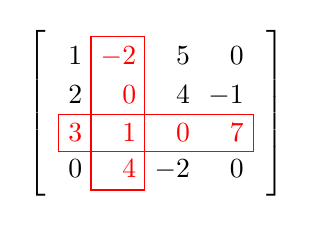
\begin{tikzpicture}[baseline=-0.5ex]%\usetikzlibrary{arrows,matrix,positioning}
		\matrix[matrix of math nodes, matrix anchor=east,
		left delimiter={[},right delimiter={]},
		every odd column/.style={anchor=base east},
		every even column/.style={anchor=base east},
		column 2/.style={color=red},
		row 3/.style={color=red},
		ampersand replacement=\&
		] (A) at (0,0)
		{
			1 \&-2 \& 5 \& 0 \\
			2 \& 0 \& 4 \&-1 \\
			3 \& 1 \& 0 \& 7 \\
			0 \& 4 \&-2 \& 0 \\
		};
		\draw[color=red] (A-1-2.north west) rectangle (A-4-3.south west);
		\draw[color=red] (A-3-1.north west) rectangle (A-3-4.south east);
		\end{tikzpicture}
		\qquad
		\xrightarrow[\text{\& 2nd Column}]{\text{Delete 3rd Row}}
		\qquad
		A_{32} &= \begin{bmatrix}1 & 5 & 0 \\ 2 & 4 &-1 \\ 0 &-2 & 0\end{bmatrix}
		\end{align*}
	\end{boxdef}
	\item Definition of Determinant
	\begin{boxdef}
		For $n\geq 2$, the \textbf{determinant} of an $n\times n$ matrix $A=[a_{ij}]$ is the sum of $n$ terms of the form $\pm a_{1j}\det A_{1j}$, with plus and minus signs alternating, where the entries $a_{11},a_{12},\ldots,a_{1n}$ are from the first row of $A$. In symbols,
		\begin{align*}
		\det A &= a_{11}\det A_{11} - a_{12}\det A_{12} + \cdots + (-1)^{1+n}a_{1n}\det A_{1n} \\
		&= \sum_{j=1}^n(-1)^{1+j}a_{1j}\det A_{1j}
		\end{align*}
	\end{boxdef}
		\begin{itemize}
			\item Notation: if $A=\begin{bmatrix}a&b\\c&d\end{bmatrix}$, then we may write $\det A = \begin{vmatrix}a&b\\c&d\end{vmatrix}$
		\end{itemize}
	\item $(i,j)$-Cofactor of $A$
	\begin{boxdef}
		\begin{multicols}{2}
			The \textbf{$\boldsymbol{(i,j)}$-Cofactor} of $A$ is the number
			$$ C_{ij} = (-1)^{i+j}\det A_{ij}. $$
			
			The factor $(-1)^{i+j}$ determines the following pattern of signs:
			$$\begin{bmatrix}[c] +&-&+&\cdots \\ -&+&-& \\ +&-&+& \\ \vdots&&&\ddots \end{bmatrix}$$
			
			\columnbreak
			
			Example: For $A=\begin{bmatrix} 1&-2&5&0 \\ 2&0&4&-1 \\ 3&1&0&7 \\ 0&4&-2&0 \end{bmatrix}$,
			\begin{align*}
			C_{32} &= (-1)^{3+2}\det A_{32} =
			-\begin{vmatrix}1&5&0\\2&4&-1\\0&-2&0\end{vmatrix}
			\end{align*}
		\end{multicols}
	\end{boxdef}
\end{itemize}

\begin{boxthm}
	\textbf{Theorem 3.1.} \\
	The determinant of a $n\times n$ matrix $A$ can be computed by a cofactor expansion across any row or down any column. The expansion across the $i$th row using the cofactors $C_{ij} = (-1)^{i+j}\det A_{ij}$ is
	$$ \det A = a_{i1}C_{i1} + a_{i2}C_{i2} + \cdots + a_{in}C_{in}. $$
	The cofactor expansion down the $j$th column is
	$$ \det A = a_{1j}C_{1j} + a_{2j}C_{2j} + \cdots + a_{nj}C_{nj}. $$
\end{boxthm}
\begin{boxthm}
	\textbf{Theorem 3.2.} \\
	If $A$ is a triangular matrix, then $\det A$ is the product of the entries on the main diagonal of $A$.
\end{boxthm}


\newpage


% SEC 3.2
\section{Properties of Determinants}

\begin{itemize}
	\item Determinants and Row Operations (Theorem 3.3)
		\begin{itemize}
			\item Use row operations to find determinants
			\begin{boxdef}
			Row reduce $A$ to an echelon form, $U$, using only row interchanges and row replacements. The number $r$ is the number of row interchanges.
			\begin{align*}
			A&\xrightarrow{\text{REF}}U &
			\det A &= (-1)^r\det U \\ &&
			&=
			\begin{cases}
			(-1)^r\cdot\left(\substack{\text{product of}\\ \text{pivots in $U$}}\right),
				\text{when $A$ is invertible} \\
			0,
				\text{when $A$ is not invertible}
			\end{cases}
			\end{align*}
			\end{boxdef}
		\end{itemize}
	\item Determinant to Assess Invertibility (Theorem 3.4)
		\begin{itemize}
			\item Add Theorem 3.4 to the Invertible Matrix Theorem
			\item Implication of Theorem 3.4: If the columns or rows of $A$ are linearly dependent, then $\det A=0$
		\end{itemize}
\end{itemize}

\begin{boxthm}
	\textbf{Theorem 3.3.}
	\textbf{Row Operations} \\
	Let $A$ be a square matrix.
	\begin{enumerate}[(a)]\itemsep0em
		\item If a multiple of one row of $A$ is added to another row to produce a matrix $B$, then $\det B=\det A$.
		\item If two rows of $A$ are interchanged to produce $B$, then $\det B=-\det A$.
		\item If one row of $A$ is multiplied by $k$ to produce $B$, then $\det B=k\cdot\det A$.
	\end{enumerate}
\end{boxthm}
\begin{boxthm}
	\textbf{Theorem 3.4.} \\
	A square matrix $A$ is invertible if, and only if, $\det A\neq 0$.
\end{boxthm}
\begin{boxthm}
	\textbf{Theorem 3.5.} \\
	If $A$ is a square matrix, then $\det A^T=\det A$.
\end{boxthm}
\begin{boxthm}
	\textbf{Theorem 3.6.}
	\textbf{Multiplicative Property} \\
	If $A$ and $B$ are $n\times n$ matrices, then $\det AB = (\det A)(\det B)$.
\end{boxthm}
\vfill


\newpage


% SEC 3.3
\section[Cramer's Rule, Volume, \& Linear Trans.]{Cramer's Rule, Volume, and Linear Transformations}

\begin{itemize}
	\item Cramer's Rule (Theorem 3.7)
		\begin{boxdef}
			Let $A_i(\vect{b})$ be the $n\times n$ matrix $A$ with the $i$th column replaced by $\vect{b}$.
			$$ \begin{bmatrix} \vect{a}_1 & \cdots & \vect{a}_{i-1} & \vect{b} & & \vect{a}_{i+1} & \cdots & \vect{a}_n \end{bmatrix} $$
		\end{boxdef}
	\begin{itemize}
		% EX here
		\item Applications to engineering: determine for what parameters a system has a unique solution
		% EX here
	\end{itemize}
	\item Inverse Formula (Theorem 3.8)
		\begin{boxdef}
			The \textbf{adjugate} (or \textbf{classical adjoint}) of a matrix $A$, denoted $\adj A$, is
			$$ \begin{bmatrix}[c]
			C_{11}&C_{21}&\cdots&C_{n1} \\
			C_{12}&C_{22}&\cdots&C_{n2} \\
			\vdots&\vdots&      &\vdots \\
			C_{1n}&C_{2n}&\cdots&C_{nn}
			\end{bmatrix},$$
			where $C_{ij}$ is the $(i,j)$-cofactor of $A$. Note that the $(i,j)$th position contains the $(j,i)$-cofactor.
		\end{boxdef}
	\item Determinants as Area or Volume (Theorem 3.9 \& 3.10)
\end{itemize}

\begin{boxthm}
	\textbf{Theorem 3.7.}
	\textbf{Cramer's Rule} \\
	Let $A$ be an invertible $n\times n$ matrix. For any $\vect{b}$ in $\R^n$, the unique solution $\vect{x}$ of $\Axb$ has entries given by
	$$ x_i = \frac{\det A_i(\vect{b})}{\det A},  \qquad  i = 1,2,\ldots, n. $$
%	\begin{align*}
%	x_i &= \frac{\det A_i(\vect{b})}{\det A}, & i &= 1,2,\ldots, n.
%	\end{align*}
\end{boxthm}
\begin{boxthm}
	\textbf{Theorem 3.8.}
	\textbf{An Inverse Formula} \\
	Let $A$ be an invertible $n\times n$ matrix. Then $ A^{-1} = \frac{1}{\det A}\adj A. $
\end{boxthm}
\begin{boxthm}
	\textbf{Theorem 3.9.} \\
	If $A$ is a $2\times 2$ matrix, the area of the parallelogram determined by the columns of $A$ is $|\det A|$. If $A$ is a $3\times 3$ matrix, the volume of the parallelpiped determined by the columns of $A$ is $|\det A|$.
\end{boxthm}
\begin{boxthm}
	\textbf{Theorem 3.10.} \\
	Let $\Tmap{2}{2}$ be the linear transformation determined by a $2\times 2$ matrix $A$. If $S$ is a parallelogram in $\R^2$, then
	\begin{align*}
	\{\text{area of } T(S)\} &= |\det A|\cdot\{\text{area of } S\}.
	\end{align*}
	If $T$ is determined by a $3\times 3$ matrix $A$, and if $S$ is a parallelpiped in $\R^3$, then
	\begin{align*}
	\{\text{volume of } T(S)\} &= |\det A|\cdot\{\text{volume of } S\}.
	\end{align*}
\end{boxthm}
\vfill


\newpage


\chapter{Vector Spaces}
% SEC 4.1
\section{Vector Spaces and Subspaces}
\begin{itemize}
	\item Vector Space
	\begin{boxdef}
		A \textbf{vector space} is a nonempty set $V$ of objects, called \textbf{vectors}, on which are defined two operations, called \textbf{addition} and \textbf{multiplication by scalers} (real numbers), subject to the ten axioms (or rules) listed below. The axioms must hold for all vectors $\vect{u}$, $\vect{v}$, and $\vect{w}$ in $V$ and for all scalars $c$ and $d$.
		\vspace{-1em}
		\begin{multicols}{2}
			\begin{enumerate}\itemsep0em
				\item $\vect{u}+\vect{v}$ is in $V$
				\item $\vect{u}+\vect{v}=\vect{v}+\vect{u}$
				\item $(\vect{u}+\vect{v}) + \vect{w} = \vect{u} + (\vect{v}+\vect{w})$
				\item There is a zero vector $\vect{0}$ in $V$ such that $\vect{u}+\vect{0}=\vect{u}$
				\item For each $\vect{u}$ in $V$, there is a vector $-\vect{u}$ in $V$ such that $\vect{u}+(-\vect{u}) = \vect{0}$
				\columnbreak
				\item $c\vect{u}$ is in $V$
				\item $c(\vect{u}+\vect{v}) = c\vect{u} + c\vect{v}$
				\item $(c+d)\vect{u} = c\vect{u} + d\vect{u}$
				\item $c(d\vect{u}) = (cd)\vect{u}$
				\item $1\vect{u} = \vect{u}$
			\end{enumerate}
		\end{multicols}
	\end{boxdef}
	\begin{boxdef}
		The 10 axioms of a vector space (listed above) imply the following helpful properties.
		\vspace{-1em}
		\begin{multicols}{3}
			\begin{enumerate}\itemsep0em
				\item $0\vect{u}=\vect{0}$
				\item $c\vect{0}=\vect{0}$
				\item $-\vect{u}=(-1)\vect{u}$
			\end{enumerate}
		\end{multicols}
	\end{boxdef}
	\begin{itemize}
		\item Examples of Vector Spaces
		\begin{itemize}
			\item $\R^n$ for any $n\in\N$.
			\item $\mathbb{S}$, the space of all doubly infinite sequences of numbers.
			$ \{y_k\} = (\ldots,y_{-2},y_{-1},y_0,y_1,y_2,\ldots) $
			\item $\Poly_n$ for $n\geq 0$, the set of polynomials of degree at most $n$.
			$ \vect{p}(t) = a_0 + a_1t + a_2t^2 + \cdots + a_nt^n $
			\item All real-valued functions defined on a set, e.g., all functions defined on $[0,1]$
		\end{itemize}
	\end{itemize}
	\item Subspaces (Theorem 4.1)
	\begin{boxdef}
		A \textbf{subspace} of a vector space $V$ is a subset $H$ of $V$ that has three properties:
		\begin{enumerate}[(a)]
			\item The zero vector is in $H$.
			\item $H$ is closed under vector addition. That is, for each $\vect{u}$ and $\vect{v}$ in $H$, the sum $\vect{u}+\vect{v}$ is in $H$.
			\item $H$ is closed under multiplication by scalars. That is, for each $\vect{u}$ in $H$ and each scalar $c$, the vector $c\vect{u}$ is in $H$.
		\end{enumerate}
	\end{boxdef}
	\begin{itemize}
		\item Examples of subspaces (and counter examples)
		\begin{itemize}
			\item The Zero Subspace, $\{\vect{0}\}$.
			\item $\Poly$, the set of all polynomials, is a subspace of the set of all real-valued functions.
			\item $\Poly_n$ is a subspace of $\Poly$
			\item $\R^2$ is \textbf{not} a subspace of $\R^3$ as vectors in $\R^3$ have to have 3 entries
		\end{itemize}
		\item The \textbf{subspace spanned by a set}, $\Span\vectsetvp$, is a subspace (Theorem 4.1)
	\end{itemize}
\end{itemize}

\begin{boxthm}
	\textbf{Theorem 4.1.} \\
	If $\vect{v}_1,\ldots,\vect{v}_p$ are in a vector space $V$, then $\Span\{\vect{v}_1,\ldots,\vect{v}_p\}$ is a subspace of $V$.
\end{boxthm}


\newpage


% SEC 4.2
\section[Null Spaces, Column Spaces, \& Linear Trans.]{Null Spaces, Column Spaces, and Linear Transformations}
\begin{itemize}
	\item Null Space (Theorem 4.2)
	\begin{boxdef}
		The \textbf{null space} of an $m\times n$ matrix $A$, written $\Nul A$, is the set of all solutions to the homogeneous equation $\Axz$. In set notation,
		$\Nul A = \{\vect{x}:\vect{x} \text{ is in } \R^n \text{ and } \Axz \}.$
	\end{boxdef}
		\begin{itemize}
			\item Find a spanning set for $\Nul A$
				\begin{enumerate}[(i)]
					\item Solve $\Ax=0$
					\item Write the solution in parametric vector form
					\item The vectors in the parametric vector form are a spanning set for $\Nul A$ \\
					Note: this spanning set is linearly independent, so the set is a basis for $\Nul A$ (see 4.3)
				\end{enumerate}
		\end{itemize}
	\item Column Space (Theorem 4.3)
	\begin{boxdef}
		The \textbf{column space} of an $m\times n$ matrix $A$, written $\Col A$, is the set of all linear combinations of the columns of $A$. If $A=\begin{bmatrix}\vect{a}_1&\vect{a}_2&\cdots&\vect{a}_n\end{bmatrix}$, then $\Col A=\Span\vectset[a]{1}{n}$, i.e., the column space is the span of the columns.
	\end{boxdef}
		\begin{itemize}
			\item $\Col A = \{ \vect{b} : \Axb \text{ for some } \vect{x} \text{ in } \R^n\}$, i.e., $\Col A$ is the range of the transformation $\vect{x}\mapsto A\vect{x}$
			\item The column space of an $m\times n$ matrix $A$ is all of $\R^m$ if, and only if, $\Axb$ has a solution for all $\vect{b}$ in $\R^m$, i.e., if the linear transformation $\vect{x}\mapsto A\vect{x}$ is onto
			\item Find a matrix $A$ with $\Col A$ equal, for example, to $W=\left\{\begin{bmatrix}6a-b\\a+b\\-7a\end{bmatrix}\right\}$
				\begin{enumerate}[(i)]
					\item Decompose $W$ into a parametric vector form using $a$ and $b$ as parameters
					\item Place the vectors in the parametric vector form into a matrix $A$ \\
					Note: These vectors may be linearly dependent---to find a basis for $\Col A$, see Theorem 4.6
				\end{enumerate}
		\end{itemize}
	\item Linear Transformations
	\begin{boxdef}
		Given a linear transformation $T:V\rightarrow W$ between vector spaces, the \textbf{kernel} (or \textbf{null space}) of $T$ is the set of all $\vect{u}$ in $V$ such that $T(\vect{u})=\vect{0}$. The \textbf{range} of $T$ is the set of all vectors in $W$ of the form $T(\vect{x})$ for some $\vect{x}$ in $V$. The kernel and range of a matrix transformation defined via a matrix $A$ are the null space and column space of $A$, respectively.
	\end{boxdef}
\end{itemize}

\begin{boxthm}
	\textbf{Theorem 4.2.} \\
	The null space of an $m\times n$ matrix $A$ is a subspace of $\R^n$. Equivalently, the set of all solutions to a system $\Axz$ of $m$ homogeneous linear equations in $n$ unknowns is a subspace of $\R^n$.
\end{boxthm}
\begin{boxthm}
	\textbf{Theorem 4.3.} \\
	The column space of an $m\times n$ matrix $A$ is a subspace of $\R^m$.
\end{boxthm}


\newpage


% SEC 4.3
\section{Linearly Independent Sets; Bases}
\begin{itemize}
	\item Basis
	\begin{boxdef}
		Let $H$ be a subspace of a vector space $V$. An indexed set of vectors $\B=\vectset[b]{1}{p}$ in $V$ is a \textbf{basis} for $H$ if
		\begin{enumerate}[(i)]
			\item $\B$ is a linearly independent set, and
			\item the subspace spanned by $\B$ coincides with $H$; that is $H=\Span\vectset[b]{1}{p}$.
		\end{enumerate}
	\end{boxdef}
		\begin{itemize}
			\item The \textbf{standard basis} for $\R^n$ is $\vectset[e]{1}{n}$ where
			\begin{align*}
			\ve1 &= \begin{bmatrix}[c] 1\\0\\0\\ \vdots \\0\end{bmatrix} &
			\ve2 &= \begin{bmatrix}[c] 0\\1\\0\\ \vdots \\0\end{bmatrix} &
			\cdots &&
			\ve{n} &= \begin{bmatrix}[c] 0\\0\\ \vdots \\0\\1\end{bmatrix}
			\end{align*}
			\item The \textbf{standard basis} for $\Poly_n$, the set of polynomials of degree no higher than $n$, is $\{1,t,t^2,\ldots, t^n\}$.
		\end{itemize}
	\item Two Views of a Basis for a Vector Space $V$
		\begin{itemize}
			\item A basis is a spanning set for $V$ that is as small as possible.
			\item A basis is a linearly independent set in $V$ that is as large as possible.
		\end{itemize}
	\item Bases for $\Nul A$ and $\Col A$
		\begin{itemize}
			\item To find a basis for $\Nul A$, write the general solution of $\Axz$ in parametric vector form. The vectors in the solution form a basis for $\Nul A$ (whenever $\Nul A \neq \{\vect{0}\}$)
			\item To find a basis for $\Col A$, select the pivot columns of $A$. (Theorem 4.6)
		\end{itemize}
\end{itemize}
\begin{boxthm}
	\textbf{Theorem 4.4.} (Similar to Theorem 1.7) \\
	An indexed set $\vectsetvp$ of two or more vectors, with $\vect{v}_1\neq 0$, is linearly dependent if, and only if, some $\vect{v}_j$ (with $j>1$) is a linear combination of the preceding vectors, $\vect{v}_1,\ldots,\vect{v}_{j-1}$.
\end{boxthm}
\begin{boxthm}
	\textbf{Theorem 4.5.}
	\textbf{The Spanning Set Theorem} \\
	Let $S=\vectsetvp$ be a set in $V$, and let $H=\Span\vectsetvp$.
	\begin{enumerate}[a.]
		\item If one of the vectors in $S$---say, $\vect{v}_k$---is a linear combination of the remaining vectors in $S$, then the set formed from $S$ by removing $\vect{v}_k$ still spans $H$.
		\item If $H\neq\{\vect{0}\}$, some subset of $S$ is a basis for $H$.
	\end{enumerate}
\end{boxthm}
\begin{boxthm}
	\textbf{Theorem 4.6.} \\
	The pivot columns of a matrix $A$ form a basis for $\Col A$.
\end{boxthm}


\newpage


% SEC 4.4
\section{Coordinate Systems}
\begin{itemize}
	\item Bases and Coordinate Systems (Theorem 4.7)
	\begin{boxdef}
		Suppose $\B=\vectset[b]{1}{n}$ is a basis for $V$ and $\vect{x}$ is in $V$. The \textbf{coordinates of $\boldsymbol{\vect{x}}$ relative to the basis $\boldsymbol{\B}$} (or the $\boldsymbol{\B}$\textbf{-coordinates of} $\boldsymbol{\vect{x}}$) are the weights $c_1,\ldots,c_n$ such that $\vect{x} = c_1\vect{b}_1 + \cdots + c_n\vect{b}_n$. We call $\vectB=\begin{bmatrix}[c] c_1 \\ \vdots \\ c_n\end{bmatrix}$ the \textbf{coordinate vector of $\boldsymbol{\vect{x}}$ (relative to $\boldsymbol{\B}$)} or the \textbf{$\boldsymbol{\B}$-coordinate vector of $\boldsymbol{\vect{x}}$}.
	\end{boxdef}
		\begin{itemize}
			\item For any $\vect{x}$ in a vector space $V$, $\vectB$ is unique (Theorem 4.7)
			\item $\vect{x}\mapsto\vectB$ is the \textbf{coordinate mapping determined by} $\boldsymbol\B$ (Theorem 4.7 and 4.8)
		\end{itemize}
	\item Graphical Interpretation of Coordinates
		\begin{itemize}
		\item The standard basis implies the usual coordinate axes---a new basis implies a new ``coordinate grid'' (see the figures below)
		\item Example: $\vect{x}=(1,6)$ below can be written as $\vectB=(-2,3)$, because $\vect{x}=-2\vect{b}_1+3\vect{b}_2$
		\begin{multicols}{2}
			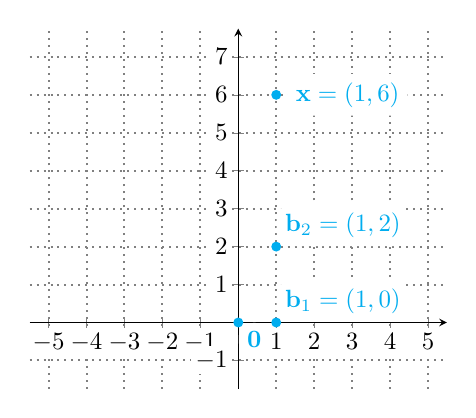
\begin{tikzpicture}[scale=.9]
			% Set u and v
			\pgfmathsetmacro{\ux}{1}
			\pgfmathsetmacro{\uy}{0}
			\pgfmathsetmacro{\vx}{1}
			\pgfmathsetmacro{\vy}{2}
			\pgfmathsetmacro{\xcoor}{1}
			\pgfmathsetmacro{\ycoor}{6}
			% Begin Axis
			\begin{axis}[axis x line=center, axis y line=middle,
			xmin=-5.5, xmax=5.5,
			ymin=-1.5, ymax=7.5,
			xtick={-5,...,5}, ytick={-1,...,7},
			ticklabel style={draw=none, inner sep=2pt, fill=white, text opacity=1},
			scale only axis, axis equal, height=2in,
			grid=major, grid style={line width=.8pt, draw=gray, dotted}]
			% Plot vectors
			\fill[cyan] (0,0) circle (2pt) node[below right, fill=white, rounded corners=0.2cm] {$\vect{0}$};
			\fill[cyan] (\ux,\uy) circle (2pt) node[above right, fill=white, rounded corners=0.2cm] {$\vect{b}_1=(\ux,\uy)$};
			\fill[cyan] (\vx,\vy) circle (2pt) node[above right, fill=white, rounded corners=0.2cm] {$\vect{b}_2=(\vx,\vy)$};
			\fill[cyan] (\xcoor,\ycoor) circle (2pt) node[right=1ex, fill=white, rounded corners=0.2cm] {$\vect{x}=(\xcoor,\ycoor)$};
			\end{axis}
			\end{tikzpicture}
			
			\columnbreak
			
			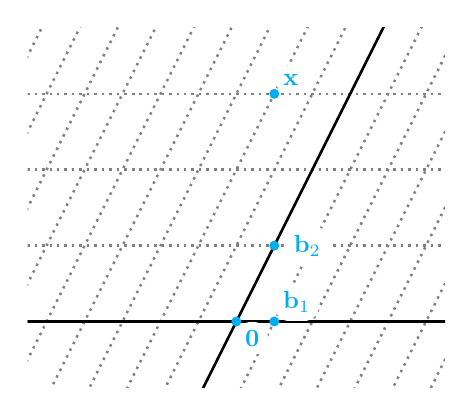
\begin{tikzpicture}[scale=.9]
			% Set u and v
			\pgfmathsetmacro{\ux}{1}
			\pgfmathsetmacro{\uy}{0}
			\pgfmathsetmacro{\vx}{1}
			\pgfmathsetmacro{\vy}{2}
			\pgfmathsetmacro{\xcoor}{1}
			\pgfmathsetmacro{\ycoor}{6}
			% Begin Axis
			\begin{axis}[axis lines=none,
			xmin=-5.5, xmax=5.5,
			ymin=-1.5, ymax=7.5,
			scale only axis, axis equal, height=2in]
			% Plot alternate coordinate system
			\foreach \yi in {-10,...,10}{
				\addplot[-, gray, dotted, line width=1pt, domain=-6.5:6.5] {(\uy/\ux)*(x-\yi*\vx)+\vy*\yi};
			}
			\foreach \xi in {-10,...,10}{
				\addplot[-, gray, dotted, line width=1pt, domain=-6.5:6.5] {(\vy/\vx)*(x-\xi*\ux)+\uy*\xi};
			}
			\addplot[-, black, line width=1pt, domain=-6.5:6.5] {(\uy/\ux)*x};
			\addplot[-, black, line width=1pt, domain=-6.5:6.5] {(\vy/\vx)*x};
			% Plot vectors
			\fill[cyan] (0,0) circle (2pt) node[below right, fill=white, rounded corners=0.2cm] {$\vect{0}$};
			\fill[cyan] (\ux,\uy) circle (2pt) node[above right, fill=white, rounded corners=0.2cm] {$\vect{b}_1$};
			\fill[cyan] (\vx,\vy) circle (2pt) node[right=1ex, fill=white, rounded corners=0.2cm] {$\vect{b}_2$};
			\fill[cyan] (\xcoor,\ycoor) circle (2pt) node[above right, fill=white, rounded corners=0.2cm] {$\vect{x}$};
			\end{axis}
			\end{tikzpicture}
		\end{multicols}
		\end{itemize}
	\item Coordinates in $\R^n$
		\begin{itemize}
			\item The \textbf{change-of-coordinates matrix} from $\B$ to the standard basis in $\R^n$, $P_\B=\begin{bmatrix}\vect{b}_1&\cdots&\vect{b}_n\end{bmatrix}$, is used to transform $\vectB$ into $\vect{x}$
			\item The \textbf{change-of-coordinates equation} is $\vect{x}=P_\B\vectB$
			\item Given $\vect{x}$ and a basis $\B$, you can find $\vectB$ by solving the system $P_\B\vectB=\vect{x}$
		\end{itemize}
	\item Coordinate Mapping (Theorem 4.8)
		\begin{itemize}
			\item A linear transformation from a vector space $V$ to a vector space $W$ that is both one-to-one and onto is called an \textbf{isomorphism} from $V$ onto $W$
			\item Any vector real vector space $V$ with a basis of $n$ vectors is isomorphic to $\R^n$---in other words, $V$ and $\R^n$ are structurally indistinguishable
			\begin{itemize}
				\item Example: $\Poly_n$ has a basis of $n+1$ vectors, $\B=\{1,t,t^2,\ldots,t^n\}$, so $\Poly_n$ is isomorphic to $\R^{n+1}$
			\end{itemize}
		\end{itemize}
\end{itemize}

\begin{boxthm}
	\textbf{Theorem 4.7.}
	\textbf{The Unique Representation Theorem} \\
	Let $\B=\vectset[b]{1}{n}$ be a basis for a vector space $V$. Then for each $\vect{x}$ in $V$, there exists a unique set of scalars $c_1,\ldots,c_n$ such that $$ \vect{x} = c_1\vect{b}_1 + \cdots + c_n\vect{b}_n. $$
\end{boxthm}
\begin{boxthm}
	\textbf{Theorem 4.8.} \\
	Let $\B=\vectset[b]{1}{n}$ be a basis for a vector space $V$. Then the coordinate mapping $\vect{x}\mapsto\vectB$ is a one-to-one linear transformation from $V$ onto $\R^n$.
\end{boxthm}


\newpage


% SEC 4.5
\section{The Dimension of a Vector Space}
\begin{itemize}
	\item Definition of Dimension (Theorem 4.10)
		\begin{boxdef}
			If $V$ is spanned by a finite set, then $V$ is said to to be \textbf{finite-dimensional}, and the \textbf{dimension} of $V$ ($\dim V$) is the number of vectors in a basis for $V$. The dimension of the zero vector space $\{\vect{0}\}$ is defined to be zero. If $V$ is not spanned by a finite set, then $V$ is \textbf{infinite-dimensional}.
		\end{boxdef}
		\begin{itemize}
			\item Every basis for a vector space $V$ is the same size (contains the same number of elements)
			\item $\dim V = \text{(Size of a basis for $V$)} $
		\end{itemize}
	\item Example: All subspaces of $\R^3$
		\begin{multicols}{2}
			\begin{itemize}\itemsep 0em
				\item 0-dimensional: the zero subspace, $\{\vect{0}\}$
				\item 1-dimensional: lines through the origin
				\item 2-dimensional: planes through the origin
				\item 3-dimensional: all of $\R^3$
			\end{itemize}
		\end{multicols}
%	\item Basis for a $p$-Dimensional Vector Space $V$ (Theorem 4.12)
%		\begin{itemize}
%			\item Any linearly independent set with exactly $p$ elements is a basis.
%			\item Any set of $p$ elements that span $V$ is a basis.
%		\end{itemize}
	\item Dimensions of Subspaces (Theorem 4.11)
		\begin{itemize}
			\item Any subspace $H$ of a finite-dimensional vector space $V$ has dimension less than (or equal to) the dimension of $V$
		\end{itemize}
	\item Dimensions of $\Nul A$ and $\Col A$
		\begin{itemize}
			\item The dimension of $\Nul A$ is the number of free variables in the equation $\Axz$
			\item The dimension of $\Col A$ is the number of pivot columns in $A$.
		\end{itemize}
\end{itemize}

\begin{boxthm}
	\textbf{Theorem 4.9.} \\
	If a vector space $V$ has a basis $\B=\vectset[b]{1}{n}$, then any set in $V$ containing more than $n$ vectors must be linearly dependent.
\end{boxthm}
\begin{boxthm}
	\textbf{Theorem 4.10.} \\
	If a vector space $V$ has a basis of $n$ vectors, then very basis for $V$ must consist of exactly $n$ vectors.
\end{boxthm}
\begin{boxthm}
	\textbf{Theorem 4.11.} \\
	Let $H$ be a subspace of a finite-dimensional vector space $V$. Any linearly independent set in $H$ can be expanded, if necessary, to a basis for $H$. Also, $H$ is finite-dimensional and $\dim H\leq\dim V$.
\end{boxthm}
\begin{boxthm}
	\textbf{Theorem 4.12.}
	\textbf{The Basis Theorem} \\
	Let $V$ be a $p$-dimensional vector space, $p\geq 1$. Any linearly independent set of vectors of exactly $p$ elements in $V$ is automatically a basis for $V$. Any set of exactly $p$ elements that spans $V$ is automatically a basis for $V$.
\end{boxthm}


\newpage


% SEC 4.6
\section{Rank}
\begin{itemize}
	\item Row Space
		\begin{itemize}
			\item If $A$ is an $m\times n$ matrix, each row can be associated with a vector in $\R^n$.
			\begin{boxdef}
				The \textbf{Row Space} of $A$, denoted $\Row A$, is the set of all linear combinations of the row vectors.
			\end{boxdef}
			\item $\Row A$ is a subspace of $\R^n$ (because each row has $n$ entries)
			\item $\Row A = \Col A^T$ (because the columns of $A^T$ are the rows of $A$)
			\item Row equivalent matrices have the same row space (Theorem 4.13)
			\item Basis for $\Row A$: row reduce $A$ to echelon form, $B$. The pivot rows of $B$ form a basis for $\Row A$
		\end{itemize}
	\item Rank (Theorem 4.14)
		\begin{boxdef}
			The \textbf{rank} of $A$ is the dimension of the column space of $A$.
		\end{boxdef}
		\begin{itemize}
			\item The Rank Theorem works because of the following equality:
			$$ \{\text{number of pivot columns}\} + \{\text{number of nonpivot columns}\} = \{\text{number of columns}\}$$
%			$$ \left\{\substack{\text{number of}\\ \text{pivot columns}}\right\} + \left\{\substack{\text{number of}\\ \text{nonpivot columns}}\right\} = \left\{\substack{\text{number of}\\ \text{columns}}\right\} $$
		\end{itemize}
\end{itemize}

\begin{boxthm}
	\textbf{Theorem 4.13.} \\
	If two matrices $A$ and $B$ are row equivalent, then their row spaces are the same. If $B$ is in echelon form, the nonzero rows of $B$ form a basis for the row space of $A$ as well as for that of $B$.
\end{boxthm}
\begin{boxthm}
	\textbf{Theorem 4.14.}
	\textbf{The Rank Theorem} \\
	The dimension of the column space and the row space of an $m\times n$ matrix $A$ are equal. This common dimension, the rank of $A$, also equals the number of pivot positions in $A$ and satisfies the equation
	$$ \rank A + \dim\Nul A = n. $$
\end{boxthm}
\begin{boxthm}
	\textbf{Theorem 2.8.}
	\textbf{The Invertible Matrix Theorem (Continued...)} \\
	Let $A$ be an $n\times n$ matrix. Then the following statements are equivalent to the statement that $A$ is an invertible matrix.
%	\begin{multicols}{2}
	\begin{enumerate}[(a)]\itemsep0em
		\setcounter{enumi}{12}
		\item The columns of $A$ form a basis for $\R^n$
		\item $\Col A = \R^n$
		\item $\dim\Col A = n$
		\item $\rank A = n$
		\item $\Nul A = \{\vect{0}\}$
		\item $\dim\Nul A = 0$
	\end{enumerate}
%	\end{multicols}
\end{boxthm}


\newpage


% SEC 4.7
\section{Change of Basis}

\begin{boxdef}
	\textbf{Some Explanation.} \\
	The standard basis for $\R^3$ is $\mathscr{E}=\left\{\begin{bmatrix}1\\0\\0\end{bmatrix},\begin{bmatrix}0\\1\\0\end{bmatrix},\begin{bmatrix}0\\0\\1\end{bmatrix}\right\}$. These vectors give us a notion of ``directions'' in $\R^3$ and are used to set up the coordinate axes we are used to. An alternate basis gives us a different set of ``directions'' to move in and effectively sets up a new coordinate system (new ``axes'') for us to use. Given two bases for $\R^3$, $\B=\{\vect{b}_1,\vect{b}_2,\vect{b}_3\}$ and $\C=\{\vect{c}_1,\vect{c}_2,\vect{c}_3\}$, we can write vectors in $\R^3$ in terms of either basis, e.g. $\vectB[x]$ or $\vectC[x]$. Translating the ``location'' of a vector from one basis is done using a change-of-coordinates matrix.
	
	From 4.4: For coordinates in $\R^n$, the \textbf{change-of-coordinates matrix} from $\B$ to the standard basis, $\E$, is the matrix $P_\B=\CoC{\B}{\E}=\begin{bmatrix}\vect{b}_1&\cdots&\vect{b}_n\end{bmatrix}.$
	$P_\B$ is used to transform $\vectB$ into $\vect{x}$ via the \textbf{change-of-coordinates equation}, $\vect{x}=P_\B\vectB$. In a similar way, we can translate between any two bases $\B$ and $\C$ using the matrix $\CoC{\B}{\C}$ described in Theorem 4.15.
\end{boxdef}

\begin{itemize}
	\item \textbf{Change-of-Coordinates Matrix from $\boldsymbol{\B}$ to $\boldsymbol{\C}$}, $\CoC{\B}{\C}$ (Theorem 4.15)
	\begin{itemize}
		\item $\CoC{\B}{\C}$ transforms $\B$-coordinate vectors to $\C$-coordinate vectors via the equation $\vectC[x]=\CoC{\B}{\C}\vectB[x]$
		\item To instead transform from $\C$ to $\B$-coordinate vectors, use $\CoC{\C}{\B} = \left(\CoC{\B}{\C}\right)^{-1}$
	\end{itemize}
	\item Ways to Determine $\CoC{\B}{\C}$
		\begin{enumerate}[(i)]
			\item If you know $\vectC[b_1],\ldots,\vectC[b_n]$, use Theorem 4.15, $\CoC{\B}{\C}=\begin{bmatrix}\vectC[b_1]&\cdots&\vectC[b_n]\end{bmatrix}$ \\ Note: this works for any vector space, not just $R^n$
			\item If bases for $\R^n$ are explicitly given, $\B=\vectset[b]{1}{n}$ and $\C=\vectset[c]{1}{n}$, row reduce:
			$$\begin{bmatrix}\vect{c}_1&\cdots&\vect{c}_n&\vect{b}_1&\cdots&\vect{b}_n\end{bmatrix} \xrightarrow{\text{RREF}} \begin{bmatrix}I_n&\CoC{\B}{\C}\end{bmatrix}$$
		\end{enumerate}
\end{itemize}

\begin{boxthm}
	\textbf{Theorem 4.15.} \\
	Let $\B=\vectset[b]{1}{n}$ and $\C=\vectset[c]{1}{n}$ be bases of a vector space $V$. Then there is a unique $n\times n$ matrix $\CoC{\B}{\C}$ such that
	$$ \vectC = \CoC{\B}{\C}\vectB. $$
	The columns of $\CoC{\B}{\C}$ are the $\C$-coordinate vectors of the vectors in the basis $\B$. That is,
	$$ \CoC{\B}{\C} = \begin{bmatrix}\vectC[b_1]&\vectC[b_2]&\cdots&\vectC[b_3]\end{bmatrix}.$$
\end{boxthm}


\newpage


\setcounter{section}{8}
% SEC 4.9
\section{Applications to Markov Chains}

\begin{itemize}
	\item STUFF
\end{itemize}

\begin{boxthm}
	\textbf{Theorem 4.18.} \\
	If $P$ is an $n\times m$ regular stochastic matrix, then $P$ has a unique steady-state vector $\vect{q}$. Further, if $\vect{x}_0$ is any initial state and $\vect{x}_{k+1}=P\vect{x}_k$ for $k=0,1,2,\ldots$, then the Markov chain $\{\vect{x}_k\}$ converges to $\vect{q}$ as $k\rightarrow\infty$.
\end{boxthm}


\newpage


\chapter{Eigenvalues \& Eigenvectors}
% SEC 5.1
\section{Eigenvectors and Eigenvalues}
\begin{itemize}
	\item Definitions
	\begin{boxdef}
		An \textbf{eigenvector} of an $n\times n$ matrix $A$ is a nonzero vector $\vect{x}$ such that $\Axlx$ for some scalar $\lambda$. A scalar $\lambda$ is called an \textbf{eigenvector} of $A$ if there is a nontrivial solution $\vect{x}$ of $\Axlx$; such an $\vect{x}$ is called an \textbf{eigenvector corresponding to $\boldsymbol{\lambda}$}.
	\end{boxdef}
		\begin{itemize}
			\item Eigenvectors must be nonzero. Eigenvalues may be zero.
		\end{itemize}
	\item Finding Eigenvalues
		\begin{itemize}
			\item For triangular matrices, the eigenvalues are the entries on the diagonal (Theorem 5.1)
			\item In general, it is not easy to find eigenvalues without first having an eigenvector (See Section 5.2)
		\end{itemize}
	\item Finding Eigenvectors (Given an Eigenvalue)
		\begin{itemize}
			\item Given an eigenvalue $\lambda$, find a nontrivial solution of $\Axlx$:
				\begin{align*}
				A\vect{x} &= \lambda\vect{x} \\
				A\vect{x} - \lambda\vect{x} &= \vect{0} \\
				A\vect{x} - \lambda I\vect{x} &= \vect{0} \\
				(A-\lambda I)\vect{x} &= \vect{0}
				\end{align*}
			\item Any nonzero vector $\vect{x}$ in the null space of a matrix of the form $(A-I\lambda)$ is an eigenvector corresponding to $\lambda$, i.e. $A\vect{x}=\lambda\vect{x}$
			\item The set of all solutions to $(A-\lambda I)\vect{x}=\vect{0}$ is called the \textbf{eigenspace} of $A$ corresponding to $\lambda$ \\
			Note: This is the null space of $(A-\lambda I)$
			\item To find a basis for an eigenspace, find a basis for the null space of $(A-\lambda I)$ (See section 4.3)
		\end{itemize}
	\item Eigenvectors and Solutions to Difference Equations
	% ADD EXAMPLE HERE
\end{itemize}

\begin{boxthm}
	\textbf{Theorem 5.1.} \\
	The eigenvalues of a triangular matrix are the entries on its main diagonal.
\end{boxthm}
\begin{boxthm}
	\textbf{Theorem 5.2.} \\
	If $\{\vect{v}_1,\ldots,\vect{v}_r\}$ are eigenvectors that correspond to distinct eigenvalues $\lambda_1,\ldots,\lambda_r$ of an $n\times n$ matrix $A$, then the set $\vectset[v]{1}{r}$ is linearly independent.
\end{boxthm}
\vfill


% SEC 5.2
\section{The Characteristic Equation}
\begin{itemize}
	\item Deriving the Characteristic Equation
	\begin{boxdef}
		Eigenvalues of an $n\times n$ matrix $A$ are scalars, $\lambda$, for which $\Axlx$ has nonzero solutions.
		\begin{enumerate}[(i)]
			\item $\Axlx$ has a nonzero solution.
				\hfill (Definition of eigenvalue)
			\item $(A-\lambda I)\vect{x} = \vect{0}$ has a nontrivial (nonzero) solution.
				\hfill (Matrix algebra)
			\item $(A - \lambda I)$ is not invertible.
				\hfill (Invertible Matrix Theorem (d))
			\item $\det(A-\lambda I) = 0$.
				\hfill (Invertible Matrix Theorem (t))
		\end{enumerate}
		A scalar $\lambda$ is an eigenvalue of an $n\times n$ matrix $A$ if, and only if, $\lambda$ satisfies the \textbf{characteristic equation}
		$$ \det(A-\lambda I) = 0. $$
		The expression $\det(A-\lambda I)$ turns out to be a polynomial of degree $n$ in the variable $\lambda$. This polynomial is called the \textbf{characteristic polynomial}. Each eigenvalue has a (algebraic) \textbf{multiplicity} which is the same as its multiplicity as a root of the characteristic equation.
		% Algebraic vs Geometric Multiplicity
		% The algebraic multiplicity of an eigenvalue λ is the power m of the term (x−λ)^m in the characteristic polynomial. The geometric multiplicity is the number of linearly independent eigenvectors you can find for an eigenvalue---this is dim Nul (A-λI), the nullity of (A-λI). When these two notions of multiplicity coincide, and only then, the matrix $A$ is diagonalizable.
		\end{boxdef}
	\begin{itemize}
		\item If an eigenvalue has multiplicity $m>1$, we typically list the eigenvalue $m$ times \\
		\textbf{Example.} If $\det(A-\lambda I)=(5-\lambda)^2(3-\lambda)(1-\lambda)$, the eigenvalues for $A$ are $\lambda=1,3,5,5$
	\end{itemize}
	\item Similarity (Theorem 5.4)
		\begin{boxdef}
			If $A$ and $B$ are $n\times n$ matrices, then $A$ is \textbf{similar} to $B$ if there is an invertible matrix $P$ such that $$P^{-1}AP=B$$ (or equivalently $A=PBP^{-1}$). We say $A$ and $B$ are \textbf{similar}. Changing $A$ into $P^{-1}AP$ is called a \textbf{similarity transformation}.
		\end{boxdef}
		\begin{itemize}
			\item \textbf{Warning:} Similar matrices have the same eigenvalues, but matrices with the same eigenvalues are not always similar.
			\textbf{Warning:} Row equivalent matrices do not usually have the same eigenvalues.
		\end{itemize}
	\item Application to Dynamical Systems
	% ADD EXAMPLE HERE
\end{itemize}

\begin{boxthm}
	\textbf{Theorem 2.8.}
	\textbf{The Invertible Matrix Theorem (Continued...)} \\
	Let $A$ be an $n\times n$ matrix. Then $A$ is invertible if, and only if:
	\begin{enumerate}[(a)]\itemsep0em
		\setcounter{enumi}{18}
		\item The number 0 is \emph{not} an eigenvalue of $A$.
		\item The determinant of $A$ is \emph{not} zero.
	\end{enumerate}
\end{boxthm}
\vspace{-1ex}
\begin{boxthm}
	\textbf{Theorem 5.3.}
	\textbf{Properties of Determinants} \\
	Let $A$ and $B$ be $n\times n$ matrices.
	\begin{enumerate}[(a)]\itemsep0em
		\item $A$ is invertible if, and only if, $\det A\neq 0$.
		\item $\det AB = (\det A)(\det B)$.
		\item $\det A^T = \det A$.
		\item If $A$ is triangular, $\det A$ is the product of the entries on the main diagonal of $A$.
		\item A row replacement operation on $A$ does not change the determinant. A row interchange changes the sign of the determinant. A row scaling also scales the determinant by the same scalar factor.
	\end{enumerate}
\end{boxthm}
\vspace{-1ex}
\begin{boxthm}
	\textbf{Theorem 5.4.}  \\
	If $n\times n$ matrices $A$ and $B$ are similar, then they have the same characteristic polynomial and hence the same eigenvalues (with the same multiplicities).
\end{boxthm}
\vfill


\newpage


% SEC 5.3
\section{Diagonalization}

\begin{itemize}
	\item Diagonalizable Matrices (Theorem 5.5)
		\begin{boxdef}
			A matrix $A$ is \textbf{diagonalizable} if $A$ is similar to a diagonal matrix $D$. That is, for some invertible matrix $P$ and diagonal matrix $D$, we have $A=PDP^{-1}$.
		\end{boxdef}
		\begin{itemize}
			\item $D$ contains all the eigenvalue information of $A$ along its main diagonal
			\item Diagonalizing a matrix lets you compute powers of the matrix efficiently: $ A^k = PD^kP^{-1} $
			\item An $n\times n$ matrix $A$ is diagonalizable if, and only if, $A$ has enough eigenvectors to form a basis of $\R^n$
		\end{itemize}
	\item Steps to Diagonalize a Matrix
		\begin{enumerate}[(i)]
			\item Find the eigenvalues of $A$
			\item Find $n$ linearly independent eigenvectors for $A$ (if this step fails, $A$ is not diagonalizable)
			\item Construct $P$ from the eigenvectors you find in step (ii)
			\item Construct $D$ by placing the corresponding eigenvectors along the diagonal \par
			To check your work, you may check that $AP=PD$
		\end{enumerate}
\end{itemize}


\begin{boxthm}
	\textbf{Theorem 5.5.}
	\textbf{The Diagonalization Theorem} \\
	An $n\times n$ matrix $A$ is diagonalizable if, and only if, $A$ has $n$ linearly independent eigenvectors.
	
	In fact, $A=PDP^{-1}$, with $D$ a diagonal matrix, if, and only if, the columns of $P$ are $n$ linearly independent eigenvectors of $A$. In this case, the diagonal entries of $D$ are eigenvalues of $A$ that correspond, respectively, to the eigenvectors in $P$.
\end{boxthm}
\begin{boxthm}
	\textbf{Theorem 5.6.} \\
	An $n\times n$ matrix with $n$ distinct eigenvalues is diagonalizable.
\end{boxthm}
\begin{boxthm}
	\textbf{Theorem 5.7.} \\
	Let $A$ be an $n\times n$ matrix whose distinct eigenvalues are $\lambda_1,\ldots,\lambda_p$.
	\begin{enumerate}[(a)]\itemsep0em
		\item The dimension of the eigenspace for $\lambda_k$ is less than or equal to the multiplicity of $\lambda_k$ (for $1\leq k\leq p$).
		\item The matrix $A$ is diagonalizable if, and only if, the sum of the dimensions of the eigenspaces equals $n$. This happens if, and only if
			\begin{enumerate*}[(i)]\itemsep0em
				\item the characteristic polynomial factors completely and
				\item the dimension of the eigenspace for each $\lambda_k$ equals the multiplicity of $\lambda_k$.
			\end{enumerate*}
		\item If $A$ is diagonalizable and $\B_k$ is a basis for the eigenspace corresponding to $\lambda_k$ for each $k$, then the total collection of vectors in $\B_1,\ldots,\B_p$ forms an eigenvector basis for $\R^n$.
	\end{enumerate}
\end{boxthm}


\begin{boxdef}
	\textbf{Some Explanation of Diagonalization (Some of this can be found in section 5.4).} \\
	Diagonalization can be viewed as a change of basis applied to a transformation. Let's say we have some $n\times n$ matrix $A$ that happens to have $n$ linearly independent eigenvectors, $\B=\{\vect{v}_1,\ldots,\vect{v}_n\}$, with associated eigenvalues $\lambda_1,\ldots,\lambda_n$. By Theorem 4.2 (The Basis Theorem), this set of eigenvectors, $\B$, is in fact a basis for $\R^n$ called an \textbf{eigenvector basis}. Denote the standard basis for $\R^n$ by $\E=\{\ve1,\ldots,\ve{n}\}$.
	
	If we form the change-of-coordinates matrix, $P=\CoC{\B}{\E}=\begin{bmatrix}\vect{v}_1&\ldots&\vect{v}_n\end{bmatrix}$, and let $D$ be the diagonal matrix with eigenvalues $\lambda_1,\ldots,\lambda_n$ down the main diagonal, we get a diagonalization: $ A = PDP^{-1}. $
	%$D=\begin{bmatrix}[c]\lambda_1&0&\ldots&0\\0&\lambda_2&\ddots&\vdots\\\vdots&\ddots&\ddots&0\\0&\ldots&0&\lambda_n\end{bmatrix}$
	
	Now, if we view $A$ as the matrix representation of a linear transformation, $\vect{x}\mapsto A\vect{x}$, and if we view $P$ and $P^{-1}$ as change-of-coordinates matrices, then we have \vspace{-1ex}
	$$ A\vect{x} = PDP^{-1}\vect{x} = \CoC{\B}{\E}D\CoC{\E}{\B}\vect{x}.$$
	What $PDP^{-1}\vect{x}$ represents, from right to left, is the following:
	\begin{enumerate}[(i)]
		\item First, $\vect{x}$ is translated into its $\B$-coordinate vector, $P^{-1}\vect{x}=\vectB[x]$.
		\item Next, the transformation of $D$ is applied to $\vectB[x]$. This is the same transformation as $A$, but in terms of the new eigenvector basis, $\B$.
		\item Finally, the transformed $\B$-coordinate vector is translated via $P$ back into the standard basis.
	\end{enumerate}
\end{boxdef}

\setcounter{section}{4}
\section{Complex Eigenvalues}
\begin{itemize}
\item A complex scalar $\lambda$ satisfies det($A-\lambda I$)=0 if and only if there is a nonzero vector $\vect{x}$ in $\mathbb{C}^n$ such that $A\vect{x}=\lambda \vect{x}$.  We call $\lambda$ a \textbf{complex eigenvalue} and $\vect{x}$ a \textbf{complex eigenvector} corresponding to $\lambda$.
\end{itemize}

\begin{boxthm}
	\textbf{Theorem 5.9.} \\
	Let $A$ be a real $2 \times 2$ matrix with a complex eigenvalue $\lambda=a-bi \; (b\neq 0)$ an associated eigenvector $\vect{v}$ in $\mathbb{C}^2$.  Then
	$$A=PCP^{-1}, \; \text{where} \; P=[\text{Re}\; \vect{v} \; \;  \; \text{Im} \; \vect{v}] \; \text{and} \; C=\begin{bmatrix} a & -b\\ b & a \end{bmatrix}$$
\end{boxthm}


\newpage


\chapter{Orthogonality \& Least Squares}
% SEC 6.1
\section{Inner Product, Length, and Orthogonality}

\begin{itemize}
	\item The Inner Product (Theorem 6.1)
	\begin{boxdef}
		The number $\vect{u}^T\vect{v}$ is called the \textbf{inner product} (or \textbf{dot product}) of $\vect{u}$ and $\vect{v}$. It is written as $\vect{u}\cdot\vect{v}$.
	\end{boxdef}
	\item The Length of a Vector
	\begin{boxdef}
		The \textbf{length} (or \textbf{norm}) of a vector $\vect{v}$ in $\R^n$ is the nonnegative scalar $\|\vect{v}\|$ defined by
		$$ \|\vect{v}\| = \sqrt{\vect{v}\cdot\vect{v}} = \sqrt{v_1^2+v_2^2+\cdots+v_n^2}. $$
	\end{boxdef}
	\begin{itemize}
		\item Note that $\|\vect{v}\|^2 = \vect{v}\cdot\vect{v}$
		\item For any scalar $c$, $\|c\vect{v}\| = |c|\|\vect{v}\|$
		\item A vector with length 1 is called a \textbf{unit vector}. To create a unit vector $\vect{u}$ form $\vect{v}$, compute $\vect{u}=\frac{1}{\|\vect{v}\|}\vect{v}$. This is called \textbf{normalizing} $\vect{v}$. We say $\vect{u}$ is \textbf{in the same direction} as $\vect{v}$.
	\end{itemize}
	\item Distance in $\R^n$
		\begin{boxdef}
			For $\vect{u}$ and $\vect{v}$ in $\R^n$, the \textbf{distance between $\boldsymbol{\vect{u}}$ and $\boldsymbol{\vect{v}}$}, written $\dist(\vect{u},\vect{v})$, is the length of the vector $(\vect{u}-\vect{v})$. That is,
			\vspace{-1em}
			$$ \dist(\vect{u},\vect{v}) = \| \vect{u}-\vect{v} \|. $$
		\end{boxdef}
	\item Orthogonal Vectors (Theorem 6.2)
		\begin{boxdef}
			Two vectors $\vect{u}$ and $\vect{v}$ are \textbf{orthogonal} (to each other) if $\vect{u}\cdot\vect{v}=0$.
		\end{boxdef}
		\begin{itemize}
			\item The zero vector, $\vect{0}$, is orthogonal to every vector
		\end{itemize}
	\item Orthogonal Complements (Theorem 6.3)
		\begin{boxdef}
			If $\vect{z}$ is orthogonal to every vector in a subspace $W$, then $\vect{z}$ is \textbf{orthogonal} to $W$. The set of all $\vect{z}$ orthogonal to $W$ is called the \textbf{orthogonal complement} of $W$, denoted $W^\perp$.
		\end{boxdef}
		\begin{itemize}
			\item A vector $\vect{x}$ is in $W^\perp$ if, and only if, $\vect{x}$ is orthogonal to every vector in a spanning set for $W$
			\item $W^\perp$ is a subspace of $\R^n$.
			\item The \textbf{4 fundamental subspaces} determined by a matrix $A$ are $\Row A$, $\Nul A$, $\Col A$, and $\Nul A^T$
		\end{itemize}
\end{itemize}


\begin{boxthm}
	\textbf{Theorem 6.1.} \\
	Let $\vect{u}$, $\vect{v}$, and $\vect{w}$ be vectors in $\R^n$, and let $c$ be a scalar. Then
	\vspace{-1.5em}
	\begin{multicols}{2}
		\begin{enumerate}[(a)]\itemsep=0em
			\item $\vect{u}\cdot\vect{v}=\vect{v}\cdot\vect{u}$
			\item $(\vect{u}+\vect{v})\cdot\vect{w}=\vect{u}\cdot\vect{w}+\vect{v}\cdot\vect{w}$
			\item $(c\vect{u})\cdot\vect{v}=c(\vect{u}\cdot\vect{v})=\vect{u}\cdot(c\vect{v})$
			\item $\vect{u}\cdot\vect{u}\geq 0$, and $\vect{u}\cdot\vect{u}=0$ if, and only if, $\vect{u}=\vect{0}$
		\end{enumerate}
	\end{multicols}
\end{boxthm}
\vspace{-1ex}
\begin{boxthm}
	\textbf{Theorem 6.2.}
	\textbf{The Pythagorean Theorem} \\
	Two vectors $\vect{u}$ and $\vect{v}$ are orthogonal if, and only if, $\|\vect{u}+\vect{v}\|^2=\|\vect{u}\|^2+\|\vect{v}\|^2$.
\end{boxthm}
\vspace{-1ex}
\begin{boxthm}
	\textbf{Theorem 6.3.} \\
	Let $A$ be an $m\times n$ matrix. The orthogonal complement of the row space of $A$ is the null space of $A$, and the orthogonal complement of the column space of $A$ is the null space of $A^T$:
	$$ (\Row A)^\perp = \Nul A \qquad \text{and} \qquad
	(\Col A)^\perp = \Nul A^T $$
\end{boxthm}


\newpage


% SEC 6.2
\section{Orthogonal Sets}

\begin{itemize}
	\item Orthogonal Sets (Theorem 6.4 \& 6.5)
	\begin{boxdef}
		A set of vectors $\vectsetvp$ in $\R^n$ is said to be an \textbf{orthogonal set} if each pair of distinct vectors from the set is orthogonal, that is, if $\vect{v}_i\cdot\vect{v}_j=0$ whenever $i\neq j$.
	\end{boxdef}
	\begin{itemize}
		\item An \textbf{orthogonal basis} for a subspace $W$ is a basis that is also an orthogonal set
	\end{itemize}
	\item Orthogonal Projection Onto the Span of a Vector (Generalized in Section 6.3)
	\begin{boxdef}
		\begin{multicols}{2}
			Suppose $\vect{u}\neq\vect{0}$ and $\vect{y}$ are vectors in $\R^n$. We wish to decompose the vector $\vect{y}$ into something in the span of $\vect{u}$ and something orthogonal to $\vect{u}$:
			$$ \vect{y} = \yhat + \vect{z}. $$
			
			\columnbreak
			
			\begin{center}
				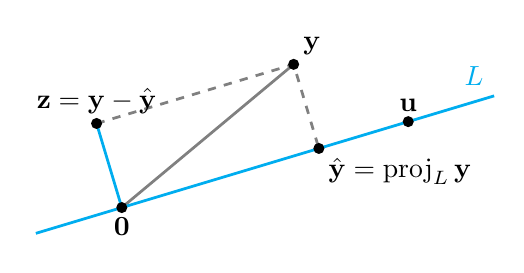
\begin{tikzpicture}[scale=1]
				% Set u and v
				\pgfmathsetmacro{\ux}{5}
				\pgfmathsetmacro{\uy}{1.5}
				\pgfmathsetmacro{\yx}{3}
				\pgfmathsetmacro{\yy}{2.5}
				\pgfmathparse{\yx*\ux+\yy*\uy}
				\pgfmathsetmacro{\ydotu}{\pgfmathresult}
				\pgfmathparse{\ux*\ux+\uy*\uy}
				\pgfmathsetmacro{\udotu}{\pgfmathresult}
				\pgfmathparse{\ydotu/\udotu*\ux}
				\pgfmathsetmacro{\yhatx}{\pgfmathresult}
				\pgfmathparse{\ydotu/\udotu*\uy}
				\pgfmathsetmacro{\yhaty}{\pgfmathresult}
				\pgfmathparse{\yx-\yhatx}
				\pgfmathsetmacro{\zx}{\pgfmathresult}
				\pgfmathparse{\yy-\yhaty}
				\pgfmathsetmacro{\zy}{\pgfmathresult}
				% Begin Axis
				\begin{axis}[axis lines=none,
				axis x line=center, axis y line=middle,
				xmin=-.5, xmax=5.5,
				ymin=-3.5, ymax=6.5,
				%	xtick={-3,...,5}, ytick={-3,...,7},
				%	xticklabels={,,}, yticklabels={,,},
				scale only axis, axis equal, % height=2in,
				gray, grid=major, grid style={line width=.5pt, draw=gray!50, dashed}]
				% Set Coordinates
				\coordinate (O) at (0,0);
				\coordinate (U) at (\ux,\uy);
				\coordinate (Y) at (\yx,\yy);
				\coordinate (YHAT) at (\yhatx,\yhaty);
				\coordinate (Z) at (\zx,\zy);
				% Connect Vectors
				\draw[line width=1pt] (O) -- (Y);
				\draw[cyan, line width=1pt] (O) -- (Z);
				\draw[dashed, line width=1pt] (Z) -- (Y) -- (YHAT);
				% Plot u and Span{u}
				\addplot[-, cyan, line width=1pt, domain=-1.5:6.5]{(\uy/\ux)*x} node[above left] {$L$};
				% Plot vectors
				\fill[black] (O) circle (2pt) node[below] {$\vect{0}$};
				\fill[black] (U) circle (2pt) node[above] {$\vect{u}$};
				\fill[black] (Y) circle (2pt) node[above right] {$\vect{y}$};
				\fill[black] (YHAT) circle (2pt) node[below right] {$\yhat=\proj_L\vect{y}$};
				\fill[black] (Z) circle (2pt) node[above] {$\vect{z}=\vect{y}-\yhat$};
				% ADD RIGHT ANGLE
				\end{axis}
				\end{tikzpicture}
			\end{center}
		\end{multicols}
		\vspace{-1em}
		The vector $\yhat$ is the \textbf{orthogonal projection} of $\vect{y}$ onto $\vect{u}$ and $\vect{z}=\vect{y}-\yhat$ is the component of $\vect{y}$ orthogonal to $\vect{u}$. Projection of $\vect{y}$ onto $\vect{u}$ is the same as projection onto the subspace spanned by $\vect{u}$. If we call $\Span\{\vect{u}\}=L$, then $\yhat=\proj_L\vect{y}$ is given by
		$$ \yhat = \proj_L\vect{y} = \frac{\vect{y}\cdot\vect{u}}{\vect{u}\cdot\vect{u}}\vect{u} $$
	\end{boxdef}
	\item Orthonormal Sets
	\begin{boxdef}
		A set $\vectset[u]{1}{p}$ is an \textbf{orthonormal} set if it is an orthogonal set of unit vectors. If $W=\Span\vectset[u]{1}{p}$, then the set is an \textbf{orthonormal basis} for $W$.
	\end{boxdef}
	\begin{itemize}
		\item An \textbf{orthogonal matrix} is a square invertible matrix $U$ such that $U^{-1}=U^T$. Since, $U^TU=I$, $U$ has orthonormal columns. Any square matrix with orthonormal columns is an orthogonal matrix.
	\end{itemize}
\end{itemize}


\begin{boxthm}
	\textbf{Theorem 6.4.} \\
	If $S=\vectset[u]{1}{p}$ is an orthogonal set of nonzero vectors in $\R^n$, then $S$ is linearly independent and hence is a basis for the subspace spanned by $S$.
\end{boxthm}
\vspace{-1ex}
\begin{boxthm}
	\textbf{Theorem 6.5.} \\
	Let $\vectset[u]{1}{p}$ be an orthogonal basis for a subspace $W$ of $\R^n$. For each $\vect{y}$ in $W$, the weights in the linear combination
	$$ \vect{y} = c_1\vect{u}_1+\cdots+c_p\vect{u}_p $$
	are given by 
	$$ c_j = \frac{\vect{y}\cdot\vect{u}_j}{\vect{u}_j\cdot\vect{u}_j} \qquad
	(\text{for } j=1,\ldots,p). $$
\end{boxthm}
\vspace{-1ex}
\begin{boxthm}
	\textbf{Theorem 6.6.} \\
	An $m\times n$ matrix $U$ has orthonormal columns if, and only if $U^TU=I$.
\end{boxthm}
\vspace{-1ex}
\begin{boxthm}
	\textbf{Theorem 6.7.} \\
	Let $U$ be an $m\times n$ matrix with orthonormal columns, and let $\vect{x}$ and $\vect{y}$ be in $\R^n$. Then
		\begin{enumerate}[(a)]\itemsep=0em
			\item $\|U\vect{x}\|=\|\vect{x}\|$
			\item $(U\vect{x})\cdot(U\vect{y}) = \vect{x}\cdot\vect{y}$
			\item $(U\vect{x})\cdot(U\vect{y}) = 0$ if, and only if, $\vect{x}\cdot\vect{y}=0$
		\end{enumerate}
\end{boxthm}


\newpage


% SEC 6.3
\section{Orthogonal Projections}

%\begin{center}
%	\begin{tikzpicture}[scale=1]
%	% Set u_1, u_2, and v
%	\pgfmathsetmacro{\uax}{5}
%	\pgfmathsetmacro{\uay}{1.5}
%	\pgfmathsetmacro{\uaz}{2}
%	\pgfmathsetmacro{\ubx}{5}
%	\pgfmathsetmacro{\uby}{1.5}
%	\pgfmathsetmacro{\ubz}{2}
%	\pgfmathsetmacro{\yx}{3}
%	\pgfmathsetmacro{\yy}{2.5}
%	\pgfmathsetmacro{\yz}{2}
%	\pgfmathparse{\yx*\uax+\yy*\uay+\yz*\uaz}
%	\pgfmathsetmacro{\ydotua}{\pgfmathresult}
%	\pgfmathparse{\uax*\uax+\uay*\uay+\uaz*\uaz}
%	\pgfmathsetmacro{\udotu}{\pgfmathresult}
%	\pgfmathparse{\ydotua/\udotu*\uax}
%	\pgfmathsetmacro{\yahatx}{\pgfmathresult}
%	\pgfmathparse{\ydotua/\udotu*\uay}
%	\pgfmathsetmacro{\yahaty}{\pgfmathresult}
%	\pgfmathparse{\ydotua/\udotu*\uaz}
%	\pgfmathsetmacro{\yahatz}{\pgfmathresult}
%	\pgfmathparse{\yx-\yahatx}
%	\pgfmathsetmacro{\zx}{\pgfmathresult}
%	\pgfmathparse{\yy-\yahaty}
%	\pgfmathsetmacro{\zy}{\pgfmathresult}
%	% Begin Axis
%	\begin{axis}[axis lines=none,
%	axis x line=center, axis y line=middle,
%	xmin=-.5, xmax=5.5,
%	ymin=-3.5, ymax=6.5,
%	%	xtick={-3,...,5}, ytick={-3,...,7},
%	%	xticklabels={,,}, yticklabels={,,},
%	scale only axis, axis equal, % height=2in,
%	gray, grid=major, grid style={line width=.5pt, draw=gray!50, dashed}]
%	% Set Coordinates
%	\coordinate (O) at (0,0);
%	\coordinate (U) at (\ux,\uy);
%	\coordinate (Y) at (\yx,\yy);
%	\coordinate (YHAT) at (\yhatx,\yhaty);
%	\coordinate (Z) at (\zx,\zy);
%	% Connect Vectors
%	\draw[line width=1pt] (O) -- (Y);
%	\draw[cyan, line width=1pt] (O) -- (Z);
%	\draw[dashed, line width=1pt] (Z) -- (Y) -- (YHAT);
%	% Plot u and Span{u}
%	\addplot[-, cyan, line width=1pt, domain=-1.5:6.5]{(\uy/\ux)*x} node[above left] {$L$};
%	% Plot vectors
%	\fill[black] (O) circle (2pt) node[below] {$\vect{0}$};
%	\fill[black] (U) circle (2pt) node[above] {$\vect{u}$};
%	\fill[black] (Y) circle (2pt) node[above right] {$\vect{y}$};
%	\fill[black] (YHAT) circle (2pt) node[below right] {$\yhat=\proj_L\vect{y}$};
%	\fill[black] (Z) circle (2pt) node[above] {$\vect{z}=\vect{y}-\yhat$};
%	% ADD RIGHT ANGLE
%	\end{axis}
%	\end{tikzpicture}
%\end{center}

\begin{itemize}
	\item Decomposition: Projection onto $W$ and Vectors in $W^\perp$ (Theorem 6.8)
	\begin{itemize}
		\item The vector $\yhat$ in Theorem 6.8 is the \textbf{orthogonal projection of $\boldsymbol{\vect{y}}$ onto $W$, denoted $\proj_W\vect{y}$.}
	\end{itemize}
	\item Best Approximations (Theorem 6.9)
	\begin{itemize}
		\item The vector $\yhat=\proj_W\vect{y}$ is called the \textbf{best approximation to $\boldsymbol{\vect{y}}$ by elements of $W$}
		\item This approximation will be used in section 6.5 for finding least-squares solutions to $\Axb$
		\item Note: If $\vect{y}$ is in $W$ already, then $\yhat=\proj_W\vect{y}=\vect{y}$, i.e. the projection of $\vect{y}$ onto $W$ is $\vect{y}$, itself
		\item The \textbf{distance from $\boldsymbol{\vect{y}}$ in $\boldsymbol{\R^n}$ to a subspace $\boldsymbol{W}$} is defined as the distance from $\vect{y}$ to the nearest point in $W$, $\yhat=\proj_W\vect{y}$
	\end{itemize}
	\item Computing Projection onto a Subspace $W$ with an Orthonormal Basis (Theorem 6.10)
\end{itemize}


\begin{boxthm}
	\textbf{Theorem 6.8.}
	\textbf{The Orthogonal Decomposition Theorem} \\
	Let $W$ be a subspace of $\R^n$. Then each $\vect{y}$ in $\R^n$ can be written uniquely in the form
	$$ \vect{y} = \yhat+\vect{z} $$
	where $\yhat$ is in $W$ and $\vect{z}$ is in $W^\perp$. In fact, if $\vectset[u]{1}{p}$ is any orthogonal basis of $W$, then
	$$ \yhat = \frac{\vect{y}\cdot\vect{u}_1}{\vect{u}_1\cdot\vect{u}_1}\vect{u}_1 + \cdots + \frac{\vect{y}\cdot\vect{u}_p}{\vect{u}_p\cdot\vect{u}_p}\vect{u}_p \qquad \text{and} \qquad \vect{z}=\vect{y}-\yhat. $$
\end{boxthm}
\begin{boxthm}
	\textbf{Theorem 6.9.}
	\textbf{The Best Approximation Theorem} \\
	Let $W$ be a subspace of $\R^n$, let $\vect{y}$ be any vector in $\R^n$, and let $\yhat$ be the orthogonal projection of $\vect{y}$ onto $W$. Then $\yhat$ is the closest point in $W$ to $\vect{y}$, in the sense that
	$$ \|\vect{y}-\yhat\| < \|\vect{y}-\vect{v}\| $$
	for all $\vect{v}$ in $W$ distinct from $\yhat$.
\end{boxthm}
\begin{boxthm}
	\textbf{Theorem 6.10.} \\
	If $\vectset[u]{1}{p}$ is an orthonormal basis for a subspace $W$ of $\R^n$, then
	$$ \proj_W\vect{y} = (\vect{y}\cdot\vect{u}_1)\vect{u}_1 + (\vect{y}\cdot\vect{u}_2)\vect{u}_2 + \cdots + (\vect{y}\cdot\vect{u}_p)\vect{u}_p. $$
	If $U=\begin{bmatrix}\vect{u}_1&\vect{u}_2&\cdots&\vect{u}_p\end{bmatrix}$, then
	$$ \proj_W\vect{y} = UU^T\vect{y} \quad \text{for all $\vect{y}$ in $\R^n$}. $$
\end{boxthm}


\newpage


% SEC 6.4
\section{The Gram-Schmidt Process}

\begin{itemize}
	\item Finding an Orthogonal Basis for a Subspace (Theorem 6.11)
		\begin{boxdef}
			The \textbf{Gram-Schmidt} process is a simple algorithm for producing an orthogonal basis for any nonzero subspace of $\R^n$. By normalizing, an orthonormal basis for the subspace may be obtained.
		\end{boxdef}
	\item Orthonormal Bases
		\begin{itemize}
			\item The Gram-Schmidt process produces an orthogonal basis for a subspace---normalize the resulting vectors to get an orthonormal basis
		\end{itemize}
	\item $QR$ Factorization (Theorem 6.12)
		\begin{enumerate}[(i)]
			\item Apply Gram-Schmidt and normalize the columns of $A$ to produce $Q=\begin{bmatrix}\vect{u}_1&\vect{u}_2&\cdots&\vect{u}_n\end{bmatrix}$.
			\item Compute $R=Q^TA$.
		\end{enumerate}
		\begin{itemize}
			\item Step (ii) above relies on Theorem 6.6 from section 6.2. Since $Q$ has orthonormal columns, $Q^TQ=I$ (by Theorem 6.6). Then we have:
			\vspace{-1em}
				\begin{align*}
					QR &= A \\
					Q^TQR &= Q^TA \\
					IR &= Q^TA \\
					R &= Q^TA
				\end{align*}
		\end{itemize}
\end{itemize}


\begin{boxthm}
	\textbf{Theorem 6.11.}
	\textbf{The Gram-Schmidt Process} \\
	Given a basis $\vectset[x]{1}{p}$ for a nonzero subspace $W$ of $\R^n$, define
	\begin{align*}
	\vect{v}_1 &= \vect{x}_1 \\
	\vect{v}_2 &= \vect{x}_2 - \frac{\vect{x}_2\cdot\vect{v}_1}{\vect{v}_1\cdot\vect{v}_1}\vect{v}_1 \\
	\vect{v}_3 &= \vect{x}_3 - \frac{\vect{x}_3\cdot\vect{v}_1}{\vect{v}_1\cdot\vect{v}_1}\vect{v}_1 - \frac{\vect{x}_3\cdot\vect{v}_2}{\vect{v}_2\cdot\vect{v}_2}\vect{v}_2 \\
	&\vdots \\
	\vect{v}_p &= \vect{x}_p - \frac{\vect{x}_p\cdot\vect{v}_1}{\vect{v}_1\cdot\vect{v}_1}\vect{v}_1 - \frac{\vect{x}_p\cdot\vect{v}_2}{\vect{v}_2\cdot\vect{v}_2}\vect{v}_2 - \ldots -  \frac{\vect{x}_p\cdot\vect{v}_{p-1}}{\vect{v}_{p-1}\cdot\vect{v}_{p-1}}\vect{v}_{p-1}.
	\end{align*}
	Then $\vectsetvp$ is an orthogonal basis for $W$. In addition
	$$ \Span\vectset{1}{k} = \Span\vectset[x]{1}{k} \qquad \text{for } 1\leq k\leq p. $$
\end{boxthm}
\begin{boxthm}
	\textbf{Theorem 6.12.}
	\textbf{The $\boldsymbol{QR}$ Factorization} \\
	If $A$ is an $m\times n$ matrix with linearly independent columns, then $A$ can be factored as $A=QR$, where $Q$ is an $m\times n$ matrix whose columns form an orthonormal basis for $\Col A$ and $R$ is an $n\times n$ upper triangular invertible matrix with positive entries on its diagonal.
\end{boxthm}


\newpage


% SEC 6.5
\section{Least-Squares Problems}

\begin{itemize}
	\item The General Least-Squares Problem
	\begin{boxdef}
		If $A$ is $m\times n$ and $\vect{b}$ is in $\R^m$, a \textbf{least-squares solution} of $\Axb$ is an $\xhat$ in $\R^n$ such that
		\vspace{-1ex}
		$$ \|\vect{b}-A\xhat\| \leq \|\vect{b}-A\vect{x}\| \qquad
		\text{for all $\vect{x}$ in $\R^n$.} $$
	\end{boxdef}
		\begin{itemize}
			\item The method of least-squares is designed to come up with approximate solutions to inconsistent systems of the form $\Axb$. If $\Axb$ cannot be solved exactly, the least-squares solution, $\xhat$, is chosen so that $A\xhat$ is as close to $\vect{b}$ as possible. If $\Axb$ is consistent, then the least-squares solution will be a real solution to the system.
			\item The distance from $\vect{b}$ to $A\xhat$, $\|\vect{b}-A\xhat\|$, is called the \textbf{least-squares error} of the approximation
			\item Since $A\vect{x}$ has to be in $\Col A$, we approximate $\Axb$ with  $\Axbhat$ where $\bhat=\proj_{\Col A}\vect{b}$
		\end{itemize}
	\item The Normal Equations (Explanation of Theorem 6.13)
		\begin{boxdef}
			Finding the least-squares solution to $\Axb$ amounts to solving $\Axbhat$ where $\bhat$ is the projection of $\vect{b}$ onto the column space of $A$. By Theorem 6.3, $\Col A$ is the orthogonal complement of $\Nul A^T$. So by Theorem 6.8, the Orthogonal Decomposition Theorem, we can write $\vect{b}=\bhat+\vect{z}$ where $\vect{z}$ is in $\Nul A^T$ and $\bhat=\proj_{\Col A}\vect{b}$. Then we have:
			\vspace{-2em}
			\begin{multicols}{2}
				\begin{align*}
				\vect{b} &= \bhat+\vect{z} \\
				A^T\vect{b} &= A^T(\bhat+\vect{z}) \\
				A^T\vect{b} &= A^T\bhat+A^T\vect{z}	& \text{(by linearity)} \\
				A^T\vect{b} &= A^T\bhat	& \text{(since $\vect{z}$ is in $\Nul A^T$)}
				\end{align*}
				\columnbreak
				
				We can use this to find a solution to $\Axbhat$ without actually computing $\bhat$ as follows:
				\begin{align*}
				A\xhat &= \bhat \\
				A^TA\xhat &= A^T\bhat \\
				A^TA\xhat &= A^T\vect{b} & (\dagger) \\
				\end{align*}
			\end{multicols}
		\vspace{-2.5em}
		\end{boxdef}
		\begin{itemize}
			\item The matrix equation $\NormEq$ represents a system of equations called the \textbf{normal equations} for $\Axb$. A solution to the normal equations $(\dagger)$ is often denoted as $\xhat$.
			\item If $A^TA$ is invertible, $\xhat$ is unique and may be computed directly (Theorem 6.14)
		\end{itemize}
	\item Alternative Calculations of Least-Squares Solutions (Theorem 6.15)
\end{itemize}


\begin{boxthm}
	\textbf{Theorem 6.13.} \\
	The set of least-squares solutions of $\Axb$ coincides with the nonempty set of solutions of the normal equations $\NormEq$.
\end{boxthm}
\vspace{-1ex}
\begin{boxthm}
	\textbf{Theorem 6.14.} \\
	Let $A$ be an $m\times n$ matrix. The following statements are logically equivalent:
	\begin{enumerate}[(a)]\itemsep=0em
		\item The equation $\Axb$ has a unique least-squares solution for each $\vect{b}$ in $\R^m$.
		\item The columns of $A$ are linearly independent.
		\item The matrix $A^TA$ is invertible.
	\end{enumerate}
	When these statements are true, the least squares solution $\xhat$ is given by
	$ \xhat = \left(A^TA\right)^{-1}A^T\vect{b}. $
\end{boxthm}
\vspace{-1ex}
\begin{boxthm}
	\textbf{Theorem 6.15.} \\
	Given an $m\times n$ matrix $A$ with linearly independent columns, let $A=QR$ be a $QR$ factorization of $A$ as in Theorem 6.12. Then, for each $\vect{b}$ in $\R^m$, the equation $\Axb$ has a unique least-squares solution, given by
	\vspace{-1em}
	\begin{align*}
	\xhat &= R^{-1}Q^T\vect{b}. &
	(\text{Numerical Note: it is usually much quicker to solve } R\xhat = Q^T\vect{b}.)
	\end{align*}
\end{boxthm}


\newpage


\chapter[Symmetric Matrices \& Quad. Forms]{Symmetric Matrices and Quadratic Forms}
% SEC 7.1
\section{Diagonalization of Symmetric Matrices}

\begin{itemize}
	\item Symmetric Matrices (Theorem 7.1-7.3)
		\begin{boxdef}
			A \textbf{symmetric matrix} is a matrix $A$ such that $A^T=A$.
		\end{boxdef}
	\item Steps to Orthogonally Diagonalize Symmetric Matrices
		\begin{itemize}
			\item An $n\times n$ matrix $A$ is said to be \textbf{orthogonally diagonalizable} if there are an orthogonal matrix $P$ (with \emph{orthonormal} columns) and a diagonal matrix $D$ such that $A=PDP^{-1}=PDP^T$.
		\end{itemize}
		\begin{enumerate}[(i)]\itemsep=0em
			\item Find the eigenvalues of $A$ 
			\item Find $n$ linearly independent eigenvectors for $A$, orthogonalize the set (if necessary), and normalize
			\item Construct $P$ from the orthonormalized eigenvectors you obtain in step (ii)
			\item Construct $D$ by placing the corresponding eigenvectors along the diagonal of $D$
		\end{enumerate}
	\item Spectral Decomposition
	\begin{itemize}
		\item The set of eigenvalues of a matrix $A$ is called the \textbf{spectrum} of $A$
		\item The spectral decomposition for $A$ can be obtained from the columns of $P$ and eigenvalues from $D$ in the orthogonal diagonalization of $A$ (see below)
	\end{itemize}
	\begin{boxdef}
	Suppose $A=PDP^{-1}$ where the columns of $P$ are orthonormal eigenvectors $\vect{u}_1,\ldots,\vect{u}_n$ of $A$ and $D$ is diagonal with corresponding eigenvalues $\lambda_1,\ldots,\lambda_n$ in the diagonal entries. Since $P^{-1}=P^T$, we have
	\vspace{-2em}
	\begin{multicols}{2}
		\begin{align*}
		A &= PDP^T \\
		&= \begin{bmatrix}\vect{u}_1&\cdots&\vect{u}_n\end{bmatrix}
		\begin{bmatrix}\lambda_1&&0\\&\ddots&\\0&&\lambda_n\end{bmatrix}
		\begin{bmatrix}[c]\vect{u}_1^T\\ \vdots\\ \vect{u}_n^T\end{bmatrix}\\
		&= \begin{bmatrix}\lambda_1\vect{u}_1&\cdots&\lambda_n\vect{u}_n\end{bmatrix}
		\begin{bmatrix}[c]\vect{u}_1^T\\ \vdots\\ \vect{u}_n^T\end{bmatrix} \\
		&= \lambda_1\vect{u}_1\vect{u}_1^T + \lambda_2\vect{u}_2\vect{u}_2^T + \cdots + \lambda_n\vect{u}_n\vect{u}_n^T.
		\end{align*}
		
		\columnbreak
		
		(The last equality uses Thm 2.10: Column-Row Expansion of Matrix Product).
		
		The final expression is called a \textbf{spectral decomposition} of $A$, because it breaks up $A$ into pieces determined by the \textbf{spectrum} (the set of eigenvalues) of $A$. Each term $\lambda_k\vect{u}_k\vect{u}_k^T$ is an $n\times n$ matrix of rank 1 (so all columns are multiples of one another). Each matrix $\vect{u}_k\vect{u}_k^T$ is a projection matrix:
		$$ (\vect{u}_k\vect{u}_k^T)\vect{x} = \proj_{\vect{u}_k}\vect{x}. $$
		%		$$ (\vect{u}_k\vect{u}_k^T)\vect{x} = \proj_{\Span\{\vect{u}_k\}}\vect{x}. $$
	\end{multicols}
	\end{boxdef}
\end{itemize}


\begin{boxthm}
	\textbf{Theorem 7.1.} \\
	If $A$ is symmetric, then any two eigenvectors from different eigenspaces are orthogonal.
\end{boxthm}
\vspace{-1ex}
\begin{boxthm}
	\textbf{Theorem 7.2.} \\
	An $n\times n$ matrix $A$ is orthogonally diagonalizable if, and only if, $A$ is a symmetric matrix.
\end{boxthm}
\vspace{-1ex}
%\begin{boxthm}
%	\textbf{Theorem 7.3.}
%	\textbf{The Spectral Theorem for Symmetric Matrices} \\
%	An $n\times n$ symmetric matrix $A$ has the following properties:
%	\begin{enumerate}[(a)]\itemsep=0em
%		\item $A$ has $n$ real eigenvalues, counting multiplicities.
%		\item The dimension of the eigenspace for each eigenvalue $\lambda$ equals the multiplicity of $\lambda$ as a root of the characteristic equation.
%		\item The eigenspaces are mutually orthogonal, in the sense that eigenvectors corresponding to different eigenvalues are orthogonal.
%		\item $A$ is orthogonally diagonalizable.
%	\end{enumerate}
%\end{boxthm}
\begin{boxthm}
	\textbf{Theorem 7.3.} % Compact Version
	\textbf{The Spectral Theorem for Symmetric Matrices} \\
	An $n\times n$ symmetric matrix $A$ has the following properties:
	\vspace{-1em}
	\begin{multicols}{2}
		\begin{enumerate}[(a)]\itemsep=0em
			\item $A$ has $n$ real eigenvalues, counting multiplicities.
			\item The dimension of the eigenspace for each eigenvalue $\lambda$ equals the multiplicity of $\lambda$ as a root of the characteristic equation.
			\item The eigenspaces are mutually orthogonal, in the sense that eigenvectors corresponding to different eigenvalues are orthogonal.
			\item $A$ is orthogonally diagonalizable.
		\end{enumerate}
	\end{multicols}
\end{boxthm}
%\vspace{-1ex}
%\begin{boxthm}
%	\textbf{Theorem 2.10.}
%	\textbf{Column-Row Expansion of $\boldsymbol{AB}$} \\
%	If $A$ is $m\times n$ and $B$ is $n\times p$, then
%	\vspace{-1em}
%	\begin{align*}
%	AB &= \begin{bmatrix}\col_1(A)&\col_2(A)&\cdots&\col_n(A)\end{bmatrix}
%	\begin{bmatrix}[c]\row_1(B)\\ \row_2(B)\\ \vdots\\ \row_n(B)\end{bmatrix}
%	= \col_1(A)\row_1(B) + \cdots + \col_n(A)\row_n(B).
%	\end{align*}
%\end{boxthm}


\newpage


% SEC 7.2
\section{Quadratic Forms}

%\begin{itemize}
%	\item Herp
%	\item Derp
%\end{itemize}


\begin{boxthm}
	\textbf{Theorem 7.4.}
	\textbf{The Principal Axes Theorem} \\
	Let $A$ be an $n\times n$ symmetric matrix. Then there is an orthogonal change of variable, $\vect{x}=P\vect{y}$, that transforms the quadratic form $\vect{x}^TA\vect{x}$ into a quadratic form $\vect{y}^TD\vect{y}$ with no cross-product term.
\end{boxthm}
\begin{boxthm}
	\textbf{Theorem 7.5.}
	\textbf{Quadratic Forms and Eigenvalues} \\
	Let $A$ be an $n\times n$ symmetric matrix. Then a quadratic form $\vect{x}^TA\vect{x}$ is:
	\begin{enumerate}[(a)]\itemsep=0em
		\item positive definite if, and only if, the eigenvalues of $A$ are all positive,
		\item negative definite if, and only if, the eigenvalues of $A$ are all negative, or
		\item indefinite if, and only if, $A$ has both positive and negative eigenvalues.
	\end{enumerate}
\end{boxthm}


\vfill
%\newpage


% SEC 7.3
\section{Constrained Optimization}

\begin{boxthm}
	\textbf{Theorem 7.6.} \\
	Let $A$ be a symmetric matrix, and define $m$ and $M$ as
	\begin{align*}
	m &= \min\{ \vect{x}^TA\vect{x}:\|\vect{x}\|=1 \}, &
	M &= \max\{ \vect{x}^TA\vect{x}:\|\vect{x}\|=1 \}.
	\end{align*}
	Then $M$ is the greatest eigenvalue $\lambda_1$ of $A$ and $m$ is the least eigenvalue of $A$. The value of $\vect{x}^TA\vect{x}$ is $M$ when $\vect{x}$ is a unit eigenvector $\vect{u}_1$ corresponding to $M$. The value of $\vect{x}^TA\vect{x}$ is $m$ when $\vect{x}$ is a unit eigenvector corresponding to $m$.
\end{boxthm}
\begin{boxthm}
	\textbf{Theorem 7.7.} \\
	Let $A$, $\lambda_1$, and $\vect{u}_1$ be as in Theorem 7.6. Then the maximum value of $\vect{x}^TA\vect{x}$ subject to the constraints
	\begin{align*}
	\vect{x}^T\vect{x} &= 1, \qquad \vect{x}^T\vect{u}_1 = 0 &
	\text{(i.e., $\|x\|=1$ and $\vect{x}$ is orthogonal to $\vect{u}_1$)}
	\end{align*}
	is the second greatest eigenvalue, $\lambda_2$, and this maximum is attained when $\vect{x}$ is an eigenvector $\vect{u}_2$ corresponding to $\lambda_2$.
\end{boxthm}
\begin{boxthm}
	\textbf{Theorem 7.8.} \\
	Let $A$ be a symmetric $n\times n$ matrix with an orthogonal diagonalization $A=PDP^{-1}$, where the entries on the diagonal of $D$ are arranged so that $\lambda_1\geq\lambda_2\cdots\lambda_n$ and where the columns of $P$ are corresponding unit eigenvectors $\vect{u}_1,\vect{u}_2,\ldots,\vect{u}_n$. Then for $k=2,\ldots,n$, the maximum value of $\vect{x}^TA\vect{x}$ subject to the constraints
	\begin{align*}
	\vect{x}^T\vect{x} &= 1, \quad
	\vect{x}^T\vect{u}_1 = 0, \quad \ldots, \quad
	\vect{x}^T\vect{u}_{k-1} = 0 &
	\text{(i.e., $\|x\|=1$ and $\vect{x}$ is orthogonal to $\vect{u}_1,\ldots,\vect{u}_{k-1}$)}
	\end{align*}
	is the eigenvalue $\lambda_k$, and this maximum is attained at $\vect{x}=\vect{u}_k$.
\end{boxthm}


\newpage


% SEC 7.4
%\setcounter{section}{3}
\section[The SVD]{The Singular Value Decomposition}

%\begin{itemize}
%	\item 
%\end{itemize}


\begin{boxthm}
	\textbf{Theorem 7.9.} \\
	Suppose $\vectsetvp$ is an orthonormal basis of $\R^n$ consisting of eigenvectors of $A^TA$, arranged so that the corresponding eigenvalues of $A^TA$ satisfying $\lambda_1\geq\cdots\geq\lambda_n$, and suppose $A$ has $r$ nonzero singular values. Then $\{A\vect{v}_1,\ldots,A\vect{v}_r\}$ is an orthogonal basis for $\Col A$, and $\rank A=r$.
\end{boxthm}
\begin{boxthm}
	\textbf{Theorem 7.10.}
	\textbf{The Singular Value Decomposition} \\
	Let $A$ be an $m\times n$ matrix with rank $r$. Then there exists an $m\times n$ matrix $\Sigma$ for which the diagonal entries in $D$ are the first $r$ singular values of $A$, $\sigma_1\geq\sigma_2\geq\cdots\geq\sigma_r>0$, and there exist an $m\times m$ orthogonal matrix $U$ and an $n\times n$ orthogonal matrix $V$ such that
	$$ A = U\Sigma V^T. $$
\end{boxthm}
\begin{boxthm}
	\textbf{Theorem 2.8.}
	\textbf{The Invertible Matrix Theorem (Concluded)} \\
	Let $A$ be an $n\times n$ matrix. Then $A$ is invertible if, and only if:
	\begin{enumerate}[(a)]\itemsep0em
		\setcounter{enumi}{20}
		\item $(\Col A)^\perp = \{\vect{0}\}$.
		\item $(\Nul A)^\perp = \R^n$.
		\item $\Row A = \R^n$.
		\item $A$ has $n$ nonzero singular values.
	\end{enumerate}
\end{boxthm}


\end{document}